\documentclass[letterpaper,12pt,oneside,final]{book}
%%
%%  Template de mémoire de maîtrise ou thèse de doctorat.
%%  Normalement, il n'est pas nécessaire de modifier ce document
%%  sauf pour changer les noms des fichiers à inclure.
%%
%%  Version: 2014-10-28
%%
%% Self added packages
\usepackage{adjustbox}
\usepackage{multirow}
\usepackage{pdflscape}
\usepackage{caption}
\usepackage[usenames]{color}
\usepackage{colortbl}
\definecolor{grey}{rgb}{0.9,0.9,0.9}
\usepackage{mdframed}
\usepackage{xr}

\usepackage{framed}
%%  Accepte les caractères accentués dans le document (UTF-8).
\usepackage[utf8]{inputenc}
%%
%% Support pour l'anglais et le français (français par défaut).
%\usepackage[cyr]{aeguill}
\usepackage{lmodern}      % Police de caractères plus complète et généralement indistinguable visuellement de la police standard de LaTeX (Computer Modern).
\usepackage[T1]{fontenc}  % Bon encodage des caractères pour qu'Acrobat Reader reconnaisse les accents et les ligatures telles que ffi.
\usepackage[frenchb,english]{babel} % le langage par défaut est le dernier de la liste, c'est-à-dire français
%%
%% Charge le module d'affichage graphique.
\usepackage{graphicx}
\usepackage{epstopdf}  % Permet d'utiliser des .eps avec pdfLaTeX.
%%
%% Recherche des images dans les répertoires.
\graphicspath{{./images/}{./dia/}{./gnuplot/}}
%%
%% Un float peut apparaître seulement après sa définition, jamais avant.
\usepackage{flafter,placeins}
%%
%% Utilisation de natbib pour les citations et la bibliographie.
\usepackage{natbib}
%%
%% Autres packages.
\usepackage{amsmath,color,soulutf8,longtable,colortbl,setspace,ifthen,xspace,url,pdflscape}
%%
%% Support des acronymes.
\usepackage[nolist]{acronym}
\onehalfspacing                % Interligne 1.5.
%%
%% Définition d'un style de page avec seulement le numéro de page à
%% droite. On s'assure aussi que le style de page par défaut soit
%% d'afficher le numéro de page en haut à droite.
\usepackage{fancyhdr}
\fancypagestyle{pagenumber}{\fancyhf{}\fancyhead[R]{\thepage}}
\renewcommand\headrulewidth{0pt}
\makeatletter
\let\ps@plain=\ps@pagenumber
\makeatother
%%
%% Module qui permet la création des bookmarks dans un fichier PDF.
%\usepackage[dvipdfm]{hyperref}
\usepackage{hyperref}
\usepackage{caption}  % Hyperlien vers la figure plutôt que son titre.
\makeatletter
\providecommand*{\toclevel@compteur}{0}
\makeatother
%%
%% Définitions spécifiques au format de rédaction de Poly.
\usepackage{MemoireThese}
%%
%% Définitions spécifiques à l'étudiant.
%% -----------------------------------
%% ---> A MODIFIER PAR L'ETUDIANT <---
%% -----------------------------------
%%
%% Commandes qui affichent le titre du document, le nom de l'auteur, etc.
\newcommand\monTitre{Recommending when Design Technical Debt Should be Self-Admitted}
\newcommand\monPrenom{C\'{e}dric}
\newcommand\monNom{Noiseux}
\newcommand\monDepartement{génie informatique et génie logiciel}
\newcommand\maDiscipline{génie informatique}
\newcommand\monDiplome{M}        % (M)aîtrise ou (D)octorat
\newcommand\anneeDepot{2017}
\newcommand\moisDepot{d\'ecembre}
\newcommand\monSexe{M}           % "M" ou "F"
\newcommand\PageGarde{N}         % "O" ou "N"
\newcommand\AnnexesPresentes{O}  % "O" ou "N". Indique si le document comprend des annexes.
\newcommand\mesMotsClef{Liste,de,mot-clés,séparés,par,des,virgules}
%%
%%  DEFINITION DU JURY
%%
%%  Pour la définition du jury, les macros suivantes sont definies:
%%  \PresidentJury, \DirecteurRecherche, \CoDirecteurRecherche, \MembreJury, \MembreExterneJury
%%
%%  Toutes les macros prennent 4 paramètres: Sexe (M/F), Prénom, Nom, Titres
\newcommand\monJury{\PresidentJury{M}{Bram}{ADAMS}{Doct.}\\
\DirecteurRecherche{M}{Giulio}{ANTONIOL}{Ph.~D.}\\
\MembreJury{M}{Foutse}{KHOMH}{Ph.~D.}}

\ifthenelse{\equal{\monDiplome}{M}}{
\newcommand\monSujet{Mémoire de maîtrise}
\newcommand\monDipl{Maîtrise ès sciences appliquées}
}{
\newcommand\monSujet{Thèse de doctorat}
\newcommand\monDipl{Philosophi\ae{} Doctor}
}
%%
%% Informations qui sont stockées dans un fichier PDF.
\hypersetup{
  pdftitle={\monTitre},
  pdfsubject={\monSujet},
  pdfauthor={\monPrenom{} \monNom},
  pdfkeywords={\mesMotsClef},
  bookmarksnumbered,
  pdfstartview={FitV},
  hidelinks,
  linktoc=all
}
%%
%% Il y a un document par chapitre du mémoire.
%%
\begin{document}
%%
%% Page de titre du mémoire.
\frontmatter
% Compte optionellement la page de garde dans la pagination.
\ifthenelse{\equal{\PageGarde}{O}}{\addtocounter{page}{1}}{}
\thispagestyle{empty}%
\begin{center}%
\vspace*{\stretch{1}}
UNIVERSITÉ DE MONTRÉAL\\
\vspace*{\stretch{1}}
\MakeUppercase{\monTitre}\\
\vspace*{\stretch{1}}
\MakeUppercase{\monPrenom~\monNom}\\
DÉPARTEMENT DE \MakeUppercase{\monDepartement}\\
ÉCOLE POLYTECHNIQUE DE MONTRÉAL\\
\vspace*{\stretch{1}}
\ifthenelse{\equal{\monDiplome}{M}}{MÉMOIRE PRÉSENTÉ}{THÈSE PRÉSENTÉE} EN VUE DE L'OBTENTION\\
DU DIPLÔME DE \MakeUppercase{\monDipl}\\
(\MakeUppercase{\maDiscipline})\\
\MakeUppercase{\moisDepot} \anneeDepot
\end{center}%
\vspace*{\stretch{1}}
\copyright~\monPrenom~\monNom, \anneeDepot.
%%
%% Identification des membres du jury.
%%
\newpage\thispagestyle{empty}%
\begin{center}%
\vspace*{\stretch{2}}
\ul{UNIVERSITÉ DE MONTRÉAL}\\
\vspace*{\stretch{1}}
\ul{ÉCOLE POLYTECHNIQUE DE MONTRÉAL}\\
\vspace*{\stretch{2}}
Ce\ifthenelse{\equal{\monDiplome}{M}}{~mémoire intitulé}{tte thèse intitulée}:\\
\vspace*{\stretch{1}}
\MakeUppercase{\monTitre}\\
\vspace*{\stretch{2}}
\end{center}%
\begin{flushleft}
présenté\ifthenelse{\equal{\monDiplome}{M}}{}{e}
par:~\ul{\mbox{\MakeUppercase{\monNom} \monPrenom}}\\
en vue de l'obtention du diplôme de:~\ul{\mbox{\monDipl}}\\
a été dûment accepté\ifthenelse{\equal{\monDiplome}{M}}{}{e} par le jury d'examen constitué de:\end{flushleft}
\vspace*{\stretch{2}}
\monJury
%%
\pagestyle{pagenumber}%
%% Dédicace
%%
%% La dédicace est un hommage que l'auteur souhaite
%% rendre à une ou plusieurs personnes de son choix.
%%
\chapter*{DEDICATION}\thispagestyle{headings}
\addcontentsline{toc}{compteur}{DEDICATION}
\begin{flushright}
  \itshape
  À mes parents, Chantal Marceau et Noel Noiseux, pour leur appui tout au long de mes études, leur écoute, leurs sacrifices et leur patience face à mes ambitions.\\
  À mes collègues de Polytechnique Montréal, Loic-Anthony Sarrazin-McCann, Cedrik Rochon, Vincent Couturier et Jean-Nicolas Dang, pour avoir été présent tout au long de mon cheminement universitaire.\\
  À mon ami Marc-Antoine Beaupré pour avoir été un confident loyal et une personne sur qui je peux toujours compter.\\
\end{flushright}
          % Dédicace du document.
% Remerciements
%
%   Grâce aux remerciements, l'auteur attire l'attention du lecteur
% sur l'aide que certaines personnes lui ont apportée, sur leurs
% conseils ou sur toute autre forme de contribution lors de la
% réalisation de son mémoire. Le cas échéant, c'est dans cette section
% que le candidat doit témoigner sa reconnaissance à son directeur de
% recherche, aux organismes dispensateurs de subventions ou aux
% entreprises qui lui ont accordé des bourses ou des fonds de
% recherche.
\chapter*{ACKNOWLEDGEMENTS}\thispagestyle{headings}
\addcontentsline{toc}{compteur}{ACKNOWLEDGEMENTS}
%
Texte.
FACULTATIF     % Remerciements.
% Résumé du mémoire.
%
%   Le résumé est un bref exposé du sujet traité, des objectifs visés,
% des hypothèses émises, des méthodes expérimentales utilisées et de
% l'analyse des résultats obtenus. On y présente également les
% principales conclusions de la recherche ainsi que ses applications
% éventuelles. En général, un résumé ne dépasse pas quatre pages.
%
%   Le résumé doit donner une idée exacte du contenu du mémoire ou de la thèse. Ce ne
% peut pas être une simple énumération des parties du document, car il
% doit faire ressortir l'originalité de la recherche, son aspect
% créatif et sa contribution au développement de la technologie ou à
% l'avancement des connaissances en génie et en sciences appliquées.
% Un résumé ne doit jamais comporter de références ou de figures.

%TOTAL = 4 pages

\chapter*{RÉSUMÉ}\thispagestyle{headings}
\addcontentsline{toc}{compteur}{RÉSUMÉ}

\setlength{\parindent}{5ex} Les \ac{TD} sont des solutions temporaires et peu optimales introduites dans le code source d'un logiciel informatique pour corriger un probl\`{e}me rapidement au d\'{e}triment de la qualit\'{e} logiciel. Cette pratique est r\'{e}pendu pour diverses raisons: rapidit\'{e} d'impl\'{e}mentation, conception initiale des composantes, connaissances faibles du projet, inexp\'{e}rience du d\'{e}veloppeur ou pression face aux dates limites. Les \ac{TD} peuvent s'av\'{e}rer utiles \`{a} court terme, mais excessivement dommageables pour un logiciel et accaparantes au niveau du temps perdu. En effet, le temps requis pour corriger des probl\`{e}me et concevoir du code de qualit\'{e} n'est souvent pas compatible avec le cycle de d\'{e}veloppement d'un projet. C'est pourquoi le sujet des \ac{TD} a \'{e}t\'{e} analys\'{e} dans de nombreuses \'{e}tudes d\'{e}j\`{a}, plus sp\'{e}cifiquement dans l'optique de les d\'{e}tecter et les identifier. \par

Une approche populaire et r\'{e}cente est d'identifier les \ac{TD} qui sont consciemment admises dans le code. La particularit\'{e}s de ces dettes, en comparaison aux \ac{TD}, est qu'elles sont explicitement document\'{e}es par commentaires et intentionnellement introduites dans le code source. Les \ac{SATD} ne sont pas rares dans les projets logiciels et ont d\'{e}j\`{a} \'{e}t\'{e} largement \'{e}tudi\'{e}es concernant leur diffusion, impact sur la qualit\'{e} logiciel, criticit\'{e}, \'{e}volution et acteurs. Diverses m\'{e}thodes de d\'{e}tection sont pr\'{e}sentement utilis\'{e}es pour identifier les \ac{SATD} mais toutes demeurent sujet \`{a}m\'{e}lioration. Par exemple, l'utilisation de mots cl\'{e}s (\emph{e.g.: hack, fixme, todo, ugly, etc.}) dans les commentaires en relation avec les dettes techniques ou l'utilisation du \ac{NLP} combin\'{e} \`{a} l'apprentissage machine. Donc, notre \'{e}tude analyse dans quelle mesure des dettes techniques ayant d\'{e}j\`{a} \'{e}t\'{e} consciemment admises (\ac{SATD}) peuvent \^{e}tre utilis\'{e}es pour fournir des recommandations aux d\'{e}veloppeurs lorsqu'ils \'{e}crivent du nouveau code. En d'autres termes, le but est d'\^{e}tre capable de sugg\'{e}rer quand admettre des dettes techniques ou quand am\'{e}liorer du nouveau code en processus de r\'{e}daction. \par

Pour atteindre ce but, une approche d'apprentissage machine a \'{e}t\'{e} \'{e}labor\'{e}e, nomm\'{e}e \ac{TEDIOUS}, utilisant comme variables ind\'{e}pendantes divers types de m\'{e}triques d'entr\'{e}es au niveau des m\'{e}thodes de mani\`{e}re \`{a} pouvoir classifier des dettes techniques de conception avec comme oracle des \ac{SATD} connus. Le mod\`{e}le a \'{e}t\'{e} entrain\'{e} et \'{e}valuer sur neuf projets Java \emph{open source} contenant des \ac{SATD} pr\'{e}c\'{e}demment \'{e}tiquet\'{e}s. En d'autres termes, notre approche vise a pr\'{e}dire pr\'{e}cis\'{e}ment les \ac{TD} dans les projets logiciels. \par

\ac{TEDIOUS} fonctionne au niveau de granularit\'{e} des m\'{e}thodes, en d'autres termes, il d\'{e}tecte si une m\'{e}thode contient une dette de conception ou non. Il a \'{e}t\'{e} con\c{c}u ainsi car les d\'{e}loppeur ont d'avantage tendance \`{a} admettre des dettes techniques au niveau des m\'{e}thodes ou des blocs de code. Les \ac{TD} peuvent \^{e}tre classifi\'{e}s selon diff\'{e}rents types: conception, requis, test, code et documentation. Les dettes de conception seulement ont \'{e}t\'{e} consid\'{e}r\'{e}es car elles forment la majorit\'{e} et analyser chaque type demanderait une analyse personnalis\'{e}e. \par

\ac{TEDIOUS} est entra\^{i}n\'{e} avec des donn\'{e}es \'{e}tiquet\'{e}es comme \'{e}tant des \ac{SATD} ou non et test\'{e} avec des donn\'{e}es sans \'{e}tiquettes. Les donn\'{e}es \'{e}tiquett\'{e}es contiennent des m\'{e}thodes marqu\'{e}es comme \'{e}tant des \ac{SATD}, obtenues \`{a} partir de neuf projets logiciels analys\'{e}s par un autre groupe de recherche utilisant une approche \ac{NLP} et valid\'{e} manuellement. Les projets sont de diff\'{e}rentes dimensions (\emph{e.g.:} number of classes, methods, comments, etc.) et contiennent diff\'{e}rentes proportions de dettes de conception. Des m\'{e}triques sont extraits des donn\'{e}es \'{e}tiquett\'{e}es: m\'{e}triques de code source, m\'{e}triques de lisibilit\'{e} et alertes g\'{e}n\'{e}r\'{e}es par des outils d'analysis statiques. Neuf m\'{e}triques de code source ont \'{e}t\'{e} retenus pour fournir un portrait de la dimension, du couplage, de la complexit\'{e} et du nombre de composantes des m\'{e}thodes. Le m\'{e}trique de lisibilit\'{e} prend en consid\'{e}ration, entre autres, les retraits, la longueur des lignes et des identifiants. Deux outils d'analyse statique ont \'{e}t\'{e} utilis\'{e}s pour cerner de faibles pratiques de codage. \par

Le pr\'{e}traitement des m\'{e}triques est appliqu\'{e} pour retirer ceux \'{e}tant superflus et garder ceux \'{e}tant les plus pertinents par rapport \`{a} la variable d\'{e}pendante. Certaines caract\'{e}ristiques sont fortement corr\'{e}l\'{e}es entre elles et il serait redondant de toutes les conserver. D'autres subissent aucune ou trop de variations dans le contexte de notre ensemble de donn\'{e}es, elles ne seraient pas utiles pour concevoir un predicteur et sont donc supprim\'{e}es \'{e}galement. De plus, les m\'{e}triques sont normalis\'{e}s pour atteindre des valeurs de performance appr\'{e}ciables au niveau de la predictions inter-projets. Cette normalisation est n\'{e}cessaire car le code source des projets varie en terme de dimensions et complexit\'{e}. Finalement, l'ensemble de donn\'{e}es est d\'{e}s\'{e}quilibr\'{e}, ce qui signifie que le nombre de m\'{e}thodes \'{e}tiquet\'{e} comme \'{e}tant un \ac{SATD} est faible. Un sur\'{e}chantillonnage a \'{e}t\'{e} appliqu\'{e} sur la classe en minorit\'{e} pour g\'{e}n\'{e}rer de nouvelles instances artificielles \`{a} partir de celles existantes. \par

Les mod\`{e}les d'apprentissage machine sont construits \`{a} partir de l'ensemble d'entrainement et les predictions sont evalu\'{e}es \`{a} partir de l'ensemble de test. Cinq types de \emph{machine learners} ont \'{e}t\'{e} test\'{e}s: Decision Trees (J48), Bayesian classifiers, Random Forests, Random Trees and Bagging with Decision Trees. Ces mod\`{e}les ont \'{e}t\'{e} retenus pour obtenir une grande vari\'{e}t\'{e} de r\'{e}sultats, provenant de diff\'{e}rents algorithmes consid\'{e}r\'{e}s comme \'{e}tant les plus appropri\'{e}s et p\'{e}cis dans le contexte de notre \'{e}tude. \par

Globalement, le but de notre \'{e}tude est d'\'{e}valuer la performance de pr\'{e}diction des \ac{SATD} selon notre approche. La vision poursuivie est de favoriser une meilleure compr\'{e}hension et maintenabilit\'{e} du code source. La perspective est d'\^{e}tre capable de sugg\'{e}rer quand admettre un \ac{TD} ayant \'{e}t\'{e} identifi\'{e} pr\'{e}c\'{e}demment. Trois questions de recherche sont abord\'{e}es: \par

\begin{itemize}
	\item \textbf{RQ1}: Comment \ac{TEDIOUS} performe dans la recommandation de \ac{SATD} intra-projet? 
	\item \textbf{RQ2}: Comment \ac{TEDIOUS} performe dans la recommandation de \ac{SATD}  inter-projet?
	\item \textbf{RQ3}: Comment un \emph{smell detector} au niveau des m\'{e}thodes se compare avec \ac{TEDIOUS}?
\end{itemize}


Pour r\'{e}pondre \`{a} \textbf{RQ1}, une validation crois\'{e}e de dix \'{e}chantillons a \'{e}t\'{e} r\'{e}alis\'{e} sur tous les projets, ce qui signifie que chaque mod\`{e}le est entrain\'{e} sur 90\% de toutes les m\'{e}thodes d'un projet et test\'{e} sur 10\% de ceux-ci.  Le processus est r\'{e}p\'{e}t\'{e} dix fois pour r\'{e}duire l'effet du hasard. Une approche similaire est suivie pour \textbf{RQ2}, un mod\`{e}le est entra\^{i}n\'{e} avec 8 projets et test\'{e} avec 1. \par

Pour \'{e}valuer le performance de \ac{TEDIOUS}, des m\'{e}triques standards tels que la p\'{e}cision, le rappel et la mesure F1 sont calcul\'{e}s sur la classe \ac{SATD}. Ces m\'{e}triques sont bas\'{e}s sur la quantit\'{e} de vrais positifs, faux positifs et faux n\'{e}gatifs. Pour compl\'{e}ter cette \'{e}valuation, la pr\'{e}cision, le \ac{MCC} et le \ac{ROC} \ac{AUC} sont calcul\'{e}s, en partie pour tenir compte du nombre de vrais n\'{e}gatifs. Ce qui est vis\'{e} comme performance des mod\`{e}les d'apprentissage est un \'{e}quilibre entre pr\'{e}cision et rappel, de sugg\'{e}rer \emph{correctement} le plus grand nombre possible de \ac{TD} \`{a} admettre. \ac{MCC} et \ac{AUC} sont des indicateurs  utiles pour r\'{e}duire l'effet du hasard. L'importance des m\'{e}triques d'entr\'{e}es est aussi consid\'{e}r\'{e}e pour \'{e}valuer les mod\`{e}les. \par

Pour r\'{e}pondre \`{a} \textbf{RQ3}, la performance d'un \emph{smell detector}, \ac{DECOR}, a \'{e}t\'{e} \'{e}valu\'{e} selon sa capacit\'{e} \`{a} classifier des m\'{e}thodes \'{e}tiquett\'{e}es \ac{SATD} comme \'{e}tant des dettes techniques. Des odeurs au niveau des m\'{e}thodes seulement ont \'{e}t\'{e} analys\'{e}es, tout comme \ac{TEDIOUS}. Finalement, quelques faux positifs et faux n\'{e}gatifs ont \'{e}t\'{e} discut\'{e} qualitativement pour exprimer les limites de notre approche. \par

























      % Résumé du sujet en français.
% Abstract
%
%   Résumé de la recherche écrit en anglais sans être
% une traduction mot à mot du résumé écrit en français.

\chapter*{ABSTRACT}\thispagestyle{headings}
\addcontentsline{toc}{compteur}{ABSTRACT}
%

TOTAL = 4 pages

VOIR PROPOSITION DE RECHERCHER

%Written in English, the abstract is a brief summary similar to the previous
%section {\selectlanguage{frenchb}(Résumé)}.  However, this section is not a
%word for word translation of the French.

          % Résumé du sujet en anglais.

{\setlength{\parskip}{0pt}
%%
%% Table des matières.
\renewcommand\contentsname{TABLE OF CONTENTS}
\tableofcontents
%%
%% Liste des tableaux.
\renewcommand\listtablename{LIST OF TABLES}
\listoftables
%%
%% Table des figures.
\renewcommand\listfigurename{LIST OF FIGURES}
\listoffigures
%%
%% Liste des annexes au besoin.
}

% Liste des sigles et abbréviations
\newcommand\abbrevname{LIST OF SYMBOLS AND ABBREVIATION}
\chapter*{\abbrevname}
\addcontentsline{toc}{compteur}{\abbrevname}
\pagestyle{pagenumber}
%
\begin{acronym}
  \acro{Acc}{Accuracy}
  \acro{ASAT}{Automated Static Analysis Tools}
  \acro{AUC}{Area Under the Curve}
  \acro{CBO}{Coupling Between Objects}
  \acro{CNN}{Convolutionnal Neural Network}
  \acro{DECOR}{DEtection \& CORrection}
  \acro{FN}{False Negative}
  \acro{FP}{False Positive}
  \acro{HIST}{Historical Information for Smell Detection}
  \acro{LM}{Long Method}
  \acro{LOC}{Lines Of Code}
  \acro{LP}{Long Parameter List}
  \acro{MCC}{Matthews Correlation Coefficient}
  \acro{MDI}{Mean Decrease Impurity}
  \acro{ML}{Machine Learner}
  \acro{NLP}{Natural Language Processing}
  \acro{OO}{Object-Oriented}
  \acro{OSS}{Open Source Software}
  \acro{Pr}{Precision}
  \acro{QMOOD}{Quality Model for Object-Oriented Design}
  \acro{Rc}{Recall}
  \acro{RNN}{Recurrent Neural Network}
  \acro{ROC}{Receiving Operating Characteristics}
  \acro{RQ}{Research Question}
  \acro{SATD}{Self-Admitted Technical Debts}
  \acro{SMOTE}{Synthetic Minority Over-sampling Technique}
  \acro{SVM}{Support Vector Machines}
  \acro{TD}{Technical Debts}
  \acro{TEDIOUS}{TEchnical Debt IdentificatiOn System}
  \acro{TN}{True Negative}
  \acro{TP}{True Positive}
  \acro{WMC}{Weighted Method Complexity}
\end{acronym}
%
\begin{longtable}{lp{5in}}
Acc			    & Accuracy\\	
ASAT		  & Automated Static Analysis Tools\\		
AUC			  & Area Under the Curve\\	
CBO			  & Coupling Between Objects\\	
CNN			  & Convolutionnal Neural Network\\	
DECOR	    & DEtection \& CORrection\\			
FN				& False Negative\\
FP				& False Positive\\
HIST		   & Historical Information for Smell Detection\\		
LM				& Long Method\\
LOC			   & Lines Of Code\\	
LP				 & Long Parameter List\\
MCC			  & Matthews Correlation Coefficient\\	
MDI			    & Mean Decrease Impurity\\	
ML				& Machine Learner\\
NLP			   & Natural Language Processing\\	
OO			   & Object-Oriented\\	
OSS			   & Open Source Software\\	
Pr				 & Precision\\
QMOOD	   & Quality Model for Object-Oriented Design\\			
Rc				 & Recall\\
RNN			   & Recurrent Neural Network\\	
ROC			  & Receiving Operating Characteristics\\	
RQ				& Research Question\\
SATD		 & Self-Admitted Technical Debt\\		
SMOTE		& Synthetic Minority Over-sampling Technique\\		
SVM			  & Support Vector Machines\\	
TD			    & Technical Debt\\	
TEDIOUS	   & TEchnical Debt IdentificatiOn System\\			
TN				& True Negative\\
TP				& True Positive\\
WMC			 & Weighted Method Complexity\\	
\end{longtable}

       % Liste des sigles et abréviations.
\ifthenelse{\equal{\AnnexesPresentes}{O}}{\listofappendices}{}
\mainmatter
% Dans l'introduction, on présente le problème étudié et les buts
% poursuivis. L'introduction permet de faire connaître le cadre de la
% recherche et d'en préciser le domaine d'application. Elle fournit
% les précisions nécessaires en ce qui concerne le contexte de
% réalisation de la recherche, l'approche envisagée, l'évolution de
% la réalisation. En fait, l'introduction présente au lecteur ce
% qu'il doit savoir pour comprendre la recherche et en connaître la
% portée.

% TOTAL = 8 pages

%%
%% BRINGING THE SUBJECT
%%
\Chapter{INTRODUCTION}\label{sec:Introduction}  

% 0.5 page

\setlength{\parindent}{5ex} In today's consumer society, products have to be designed and ready to hit the market as fast as possible, in order to stand out from other similar products and generate revenues. This pressure to produce can affect the quality, maintainability and functionality of the design. In software engineering, the repercussion of this mindset can be, in a certain way, measured with the amount of technical debts present in a project. The problem is that these \ac{TD} can frequently go unnoticed if they are not admitted. In fact, studies have been conducted on technical debts that are "self-admitted", where developers comment why such code represents an issue or a temporary solution. In a similar vein, the subject of this thesis is to study how previously self-admitted technical debts can be used to recommend when to admit newly introduced technical debts.

%%
%%  CONCEPTS DE BASE
%%
\section{Basic Concepts and Definitions}  

% environ 3 pages

\setlength{\parindent}{5ex} Technical debts are temporary and less than optimal solutions introduced in the code. They are portions of code that still need to be worked on even though they accomplish their purpose. \citet{Cunningham:1992:WPM:157709.157715} first described technical debts as "not quite right code which we postpone making it right". For example, \ac{TD} can be workarounds which don't follow good coding practices, poorly structured code or hard-to-read code. By definition, technical debts don't typically cause errors or prevent the code from working but they can in some circumstances. However, various reasons can motivate the introduction of technical debts: to rapidly fix an issue, because the development team is at early stages of conception, because of a lack of comprehension, skills or experience \citep{Suryanarayana20151}. \par

\ac{TD} are introduced throughout the whole conception timeline and under various forms, partly because writing quality code is not always compatible with the standard development life cycle \citep{brown2010managing}. That is why an ontology and landscape were proposed by \citet{alves2014towards} and \citet{izurieta2012organizing} to better define the subject. In this ontology, design, requirement, code, test and documentation debts represent the main branches of the classification tree, where each branch can be linked to a specific development stage and to specific criteria. For example, \emph{design debt} "refers to debt that can be discovered by analyzing the source code by identifying the use of practices which violated the principles of good object-oriented design (e.g. very large or tightly coupled classes)" \citep{alves2014towards}. \par

Other studies investigated the perception of developers on technical debts. \citet{Ernst:2015:MMI:2786805.2786848} found that the most important source of \ac{TD} are architectural decisions, that recognizing the phenomenon is essential for communication and that there is a lack of tools to manage those debts. Additionally, software project teams recognize that this issue is unavoidable and necessary \citep{lim2012balancing} and that they cause a lot of problems. For example, slower conception and execution of the software product \citep{allman2012managing}, diminished software maintainability and quality \citep{wehaibi2016examining,zazworka2011investigating}, and higher production costs \citep{guo2011tracking}. \par

Frequently, \ac{TD} are introduced consciously and explicitly by developers. In those cases, we say that they are "self-admitted" and explained in comments, describing what is wrong with the related block of code \citep{PotdarS14}. Like technical debts, SATD are encountered in most software projects. It was found that 31\% of files contain \ac{SATD}, that they remain in the source code for a long period of time and that experienced developers are more prone to introducing them \citep{PotdarS14}. This proves that a proper management tool is required to deal with this issue, and that unexperienced developers would greatly benefit from such support to decide when code should be reworked and documented as \ac{TD}. The disparity between the experienced and unexperienced workers may also lie in the fact that the unexperienced ones don't want to admit their faults in order to maintain a positive image towards their superiors. \par

\citet{BavotaR16} found that there is no clear correlation between code quality and \ac{SATD}. Code quality metrics such as \ac{WMC}, \ac{CBO} and Buse and Weimer Readability \citep{Buse:tse2010} were computed and analyzed to reach this conclusion. However, the primary purpose of this work was not to evaluate this relationship but rather to establish a taxonomy of \ac{TD}. Some threats to the validity of their results could also be made concerning the number of manually analyzed \ac{SATD} and the level at which the metrics were computed (class-level). A finer analysis would have been required because a single class can contain methods of different lengths, complexity, cohesion, coupling and readability. This same study found an average of 51 instances of \ac{SATD} (0.3\% of all comments) in the analyzed projects, that the developer who introduces a \ac{TD} is generally the same that fixes it and that they aren't all fixed during the development life cycle. \par


%%
%% ELEMENTS DE LA PROBLEMATIQUE
%%
\section{Elements of the Problematic}  

% environ 3 pages

It is pretty clear that technical debts account for a lot of issues in the development of software applications. They have been extensively analyzed and classified in order to have a better understanding of their impact. However, the identification, as much as the \emph{correct} identification of \ac{SATD}, remains a struggle for researchers and developers. Current methods can obtain up to 25\% of their total predictions as false positives \citep{BavotaR16}. This means that a quarter of all automatically identified \ac{TD} are not really technical debts. Consequently, conclusions made by studies using these results could be erroneous considering the high level of false technical debts. 

Additionally, many strategies can be employed to reduce the number of TD and fix them: take your time when implementing a solution, code refactoring, continuous tracking of \ac{TD}, proactiveness in fixing debts, etc. \citep{Ambler} However, they are not highly effective and frequently rely on the willingness of developers to fix the problem and their general knowledge. \par

To cope with these low accuracy values, various approaches have been proposed to improve the detection of \ac{TD}. One of them is to identify comment patterns that relate to self-admitted technical debts \citep{PotdarS14}. Potdar \emph{et al.} manually went through 101 762 comments to determine them, which lead to the identification of 62 \ac{SATD} patterns, for example, \emph{hack, fixme, is problematic, this isn't very solid, probably a bug}. The main issue with this approach is the manual process behind it, which introduces human errors and subjectivity. Another approach proposed by \citet{MaldonadoNLP} is to use machine learning techniques combined with \ac{NLP} to automatically identify \ac{SATD} using source code comments. This idea is promising because it does not heavily depend on the manual classification of source code comments and in fact, it outperforms the previous approach. Manual classification is still required to build the training set for the NLP classifier but the model built from this dataset can then be used to automatically identify \ac{SATD} in any project, making irrelevant any further manual analysis. \par

It is important to mention that our research does not revolve on proposing a new technical debts detection method using information contained in comments, but rather using these identified SATD as a base for our recommendation tool. Consequently, the proper classification of \ac{SATD} methods used by \ac{TEDIOUS} will directly affect its performance. 

To properly establish the problematic of this thesis and prior to designing our approach, several research questions have to be addressed. The main one can be defined like this:  \par

\begin{center}
\begin{framed}
	\noindent How can we identify and detect technical debts in a software project using source code features and known self-admitted technical debts with a machine learning approach?
\end{framed}
\end{center}

Consequently, in the quest of helping programmers, we designed and developed TEDIOUS, a machine learning inspired recommendation systems that uses manually labeled training data to detect method-level technical debts. The goal of this thesis is then to assess the performance of TEDIOUS in recommending SATD. Three other high-level research questions can be derived from the main one:

\begin{center}
\begin{framed}
	 \noindent How does \ac{TEDIOUS} work for recommending \ac{SATD} within project? \\
	 How does \ac{TEDIOUS} work for recommending SATD across projects? \\
	 How would a method-level smell detector compare with \ac{TEDIOUS}?
\end{framed}
\end{center}
	
The evaluation goal can be addressed by these questions. Firstly, we want to evaluate the detection performance of a model trained with features from the source code of a specific system on himself. Secondly, we want to perform a similar performance evaluation on a model trained with features from several systems on another unrelated system. Finally, we want to compare the detection performance of TEDIOUS with other popular smell detectors.

Our approach is based on the hypothesis that current methods to detect technical debts are limited and inefficient, and that a new approach could be beneficial to the improvement of detection performance. We also think that manual analysis and human subjectivity is detrimental to the efficiency of current methods. Consequently, we believe that a well-crafted machine learning approach could lead to better results and performance values in identifying technical debts and recommending when they should be self-admitted. \par

%%
%% OBJECTIFS DE RECHERCHE
%%
\section{Research Objectives}  

% 0.5 page

\begin{center}
\begin{framed}
	\noindent The objective of this research is to design a machine learning approach that uses as independent variables various kinds of source code features, and as dependent variables the knowledge of previously self-admitted technical debts, to train machine learners in recommending to developers when a technical debt should be admitted.
\end{framed}
\end{center}

As mentioned previously, the purpose of this thesis is not to propose a novel method to identify SATD from source code comments using patterns or \ac{NLP} \citep{MaldonadoNLP,PotdarS14}. It is more about using these classified SATD comments to build our labeled dataset consisting of methods' source code information and metrics to identify possible technical debts to self-admit. \par
 
The main objective can be divided in two application scenarios. Firstly, tracking and managing technical debts is considered important but lacking in the industry \citep{Ernst:2015:MMI:2786805.2786848}. Consequently, \ac{TEDIOUS} could be used to encourage developers to self-admit \ac{TD} in order to easily track and fix the issues later. This is particularly true for junior developers, who are less prone to self-admitting than experienced ones \citep{PotdarS14}. Secondly, our tool could be used as an alternative, or a complement, to existing smell detectors in proposing improvements to source code. In other words, \ac{TEDIOUS} could act as a tracking, managing and improvement tool for software projects. \par

%%
%% OBJECTIFS DE DESIGN
%%
\section{Design Objectives} 

Five research objectives can be achieved by following this design methodology. The first one aims at \emph{defining and extracting relevant features from methods}. These features are characteristics that describe each method. Contrary to previous studies \citep{BavotaR16}, \ac{TEDIOUS} works at method-level rather than class-level because we found that \ac{SATD} comments are more frequently related to methods or blocks of code. We investigated a set of method structural metrics, a method readability metric and warning raised by static analysis tools. \par

The second specific objective aims at \emph{identifying self-admitted technical debts}. Only one type of technical debt is considered for various reasons, the design debt. Firstly, it is the most common type of \ac{TD} \citep{MaldonadoNLP}. Secondly, the other types (requirement, code, test and documentation) would require a different analysis and other training features. However, these types are planned to be analyzed in our future work. To identify SATD methods, TEDIOUS reuses knowledge of manually labeled TD, metrics, and static analysis warnings. In fact, the training set was extracted from the manually labeled corpus of 9 open source Java projects provided by \citet{MaldonadoNLP}.

The third specific objective aims at \emph{preprocessing the features}. Strongly correlated features are cleaned up to remove redundancy, metrics that don't vary or vary too much are removed, a normalization is applied to take into account the different nature of projects and the training set is balanced by oversampling the small number of \ac{SATD} tagged methods. \par

The fourth specific objective aims at \emph{building and applying machine learning models}. Five machine learners are trained and tested, performing \ac{SATD} prediction within project and across projects. The five retained ML are: Decision Trees (J48), Bayesian classifiers, Random Forests, Random Trees and Bagging with Decision Trees. \par

We could add another objective which aims at \emph{improving the first TEDIOUS approach}. To do so, a Convolutionnal Neural Network is designed and implemented, using the source code itself as the independent variable. It is tested using the same dataset, within project, and with different independent variable configurations: with, without or partially with comments. Results show improvement compared to the previous approach, in terms of precision, recall, $F_1$ score and accuracy.

%%
%% PLAN DU MEMOIRE
%%
\section{Thesis Overview}  

% 0.5 page

\paragraph{Chapter 2: Literature Review}
The literature review provides a current state-of-the-art overview of the knowledge on technical debts and other related topics. It summarizes relevant information extracted from previous studies concerning four main topics: relationship between technical debt and source code metrics, self-admitted technical debt, code smell detection and automated static analysis tools.

\paragraph{Chapter 3: The Approach and Study Definition}
The approach followed is thoroughly described in several steps. The types of features are described and the way they are extracted is explained. The provenance and identification of the \ac{SATD} tagged comments are shared. The preprocessing that is performed on features is demystified and justified. The machine learning models chosen are revealed as well as their configuration. As for the study definition, the dataset characteristics (number of files, classes, comments, etc.) are shared for each project and the analysis method (cross validation, accuracy, precision, recall, F$_{1}$ score, \ac{MCC}, \ac{ROC}, \ac{AUC}) explained.

\paragraph{Chapter 4: Analysis of Study Results and Threats to Validity}
The study results are analyzed based on each research question: performance for within project prediction, performance for across-project prediction and comparison with a method-level smell detector. Results indicate that within project prediction achieves at best 50\% precision and 52\% recall. Improvement is made for across projects prediction where prediction achieves at best 67\% precision and 55\% recall. The best machine learner turned out to be Random Forest. It was also found that \ac{SATD} predictions made by \ac{TEDIOUS} only weakly relate to method-level code smells. A qualitative discussion on false positives and negatives is also proposed. Following the results analysis, several threats to validity are shared: construct, internal, conclusion and external validity threats.

\paragraph{Chapter 5: Convolutionnal Neural Network with Comments and Source Code} This chapter describes an updated approach to detect \ac{TD} to self-admit and its preliminary results. First, the \ac{CNN} characteristics and features are described. Secondly, the approach is explained: the features used, the identification of \ac{SATD}, the use of word embeddings and the way the \ac{CNN} is built and applied to the context of our research. Thirdly, the study definition is described: the characteristics of the dataset and the analysis method. Finally, the study results are analyzed based on three prediction contexts: source code with comments, without comments and partially with comments. Various \ac{CNN} configurations are also analyzed. Results indicate that source code with comments obtains the best performance values. It achieves 84.06\% precision, 74.50\% recall and 98.89\% accuracy.









       % Introduction au sujet de recherche.
\Chapter{LITERATURE REVIEW}\label{sec:RevLitt}

% TOTAL = 4 pages

\setlength{\parindent}{5ex}The literature related to this thesis can be divided in four topics, which will be summarized in this chapter. The first one addresses the relationship between technical debt and source code metrics. The second defines what are self-admitted technical debts. The third topic describes code smell detection approaches and the last one covers the usage of automated static analysis tools.

\section{Relationship Between Technical Debt and Source Code Metrics}

Many researchers have tried to link technical debts, more specifically design and code types, to source code metrics. \citet{marinescu2012assessing} proposed an approach based on a technique for detecting design flaws and built on top of a set of metric rules capturing coupling, cohesion and encapsulation. \citet{griffith2014correspondence} empirically validated the relationship between \ac{TD} and software quality models. Three \ac{TD} detection methods were compared with \ac{QMOOD} \citep{bansiya2002hierarchical} and only one of them had a strong correlation to quality attributes, namely reusability and understandability. A larger study was performed by \citet{fontana2016technical} where they analyzed how five different tools detect technical debts, their principal features, differences and missing aspects. They focused on the impact of design smells on code debt to give advices on which design debt should be prioritized for refactoring. These tools all took into account metrics, smells, coding rules and architecture violations. However, there was only a limited agreement among tools and they still ignored some important pieces of information.

\section{Self-Admitted Technical Debt}

Many studies have been conducted in order to describe and classify the nature of self-admitted technical debts. \citet{PotdarS14} investigated technical debts in the source code of open source projects and they found out that developers frequently self-admit \ac{TD} they introduce, explaining in the form of comments why these particular blocks of code are temporary and need to be reworked. They are some of the first to acknowledge the existence of \ac{SATD} and to propose a detection method using pattern matching in source code comments. \citet{MaldonadoS15} analyzed developers' comments in order to define and quantify different types of \ac{SATD}. An approach similar to the one of \citet{PotdarS14} is followed, which is using pattern matching to classify \ac{SATD} into five types: design, defect, documentation, requirement and test. It was found that design debts are the most common, making up between 42\% and 84\% of all comments in software projects. \par

\citet{BavotaR16} performed a large-scale empirical study on self-admitted technical debts in open source projects. They studied their diffusion and evolution, the actors involved in managing \ac{SATD} and the relationship between \ac{SATD} and software quality. They showed that there is on average 51 instances of \ac{SATD} per system, that code debts are the most frequent, followed by defect and requirement debts, that the number of instances increases over time because they are not fixed by developers, and that they normally survive for a long time. Like \citet{griffith2014correspondence}, they found no real correlation between \ac{SATD} and quality metrics (\ac{WMC}, \ac{CBO}, Buse and Weimer readability). \par

\citet{wehaibi2016examining} also studied the relation between self-admitted technical debts and software quality. Their approach is based on investigating if more defects are present in files with more \ac{SATD}, if \ac{SATD} changes are more likely to cause the emergence of future defects and whether changes are more difficult to perform or not. They found that no real trend could be made between \ac{SATD} and defects, that \ac{SATD} changes did not introduce more future defects than no-\ac{SATD} changes but that they are indeed more difficult to perform. \par

\citet{MaldonadoNLP} recently proposed a new approach based on \ac{NLP} techniques to detect self-admitted technical debts, more specifically design and requirement debts. They extracted comments from ten open source projects, cleaned them to remove irrelevant ones and manually classified them into the different types of \ac{SATD}. This dataset was then used as the training set for a maximum entropy classifier. It turned out that the model could accurately identify \ac{SATD} and outperform the pattern matching method of \citet{PotdarS14}. Comments mentioning sloppy or mediocre source code were the best indicators of design debts and comments related to partially implemented requirement were the best for requirement debts. \par

Contrary to previous studies, the goal of TEDIOUS is to detect methods that are TD prone. This is to say differently from \citet{MaldonadoS15}, our goal is not to classify comments but rather to categorize methods based on those classified comments.

\section{Code Smell Detection}

Several approaches to detect code smells have been proposed in today's literature: \citet{Travassos99-ACM-Inspections} developed reading techniques to guide developers in identifying defects in \ac{OO} designs, \citet{Marinescu04-ICSM-DetectionStrategies} formulated metrics-based rules as a detection strategy that can capture poor design practices and \citet{Munro05-BadSmellIdentification} used software metrics to characterize bad smells. Others such as \citet{moha2010decor} proposed \ac{DECOR}, an approach using rules and thresholds on various metrics to detect smells. This smell detector is in fact used to compare its performance with TEDIOUS. 

Many detection techniques rely on structural information, however, \citet{PalombaBPOPL15} exploited change history information to propose \ac{HIST}, a smell detector that identifies instances of five different code smells, with promising results. On the other hand, \citet{FokaefsTSC11} used graph matching to propose JDeodorant, an Eclipse plugin that automatically applies refactoring on "God Classes". Using graph matching also, \citet{Tsantalis:tse2009} proposed a methodology recommending "Move Method" refactoring opportunities for "Feature Envy" bad smells to reduce coupling and increase cohesion. 

Machine learning techniques are also popular. \citet{fontana2016comparing} compared and experimented with 16 different machine learning algorithms to detect code smells, \citet{khomh2009bayesian} proposed a Bayesian approach to detect code and design smells, and \citet{maiga2012support} proposed SVMDetect, a new approach to detect anti-patterns using a \ac{SVM} technique. \par 

TEDIOUS is different from these previous approaches for two main reasons. Firstly, they use structural or historical information and metrics from the code to detect smells. However, in addition to these characteristics, we also use feedback provided by developers, in the form of \ac{SATD} comments which leads to the identification of technical debts. Secondly, we also use warnings generated by \ac{ASAT} to portray an even better representation of the source code quality. \par 

\section{Automated Static Analysis Tools}

The subject of automated static analysis tools have already been widely covered to analyze its benefits on the development of software projects. To understand the actual gains provided by automated static analysis tools, \citet{couto2013static} studied the correlation and correspondence between post-release defects and warnings issued by the bug finding tool FindBugs. Only a moderate correlation and no correspondence were found between defects and raised warnings. On the other hand, three \ac{ASAT} were evaluated by \citet{wedyan2009effectiveness} showing that they could successfully recommend refactoring opportunities to developers. \citet{ayewah2007evaluating} also evaluated an FindBugs, its performance was measured to quantify its accuracy and the value of warnings raised. They found that warnings were mostly considered relevant by developers and that they were willing to make the appropriate modifications to fix the issues. \citet{BellerBMZ16} performed an evaluation of several ASAT on an even larger scale. They found that the use of \ac{ASAT} is widespread but no strict usage policy is imposed in software projects. Generally, the automated static analysis tools are used with their default configuration, only a small amount is significantly changed. Also, \ac{ASAT} configurations experience little to no modifications over time. \par 

Many of the mentioned studies share common views and purposes with our research and \ac{TEDIOUS}. However, as far as we know, TEDIOUS stands out because it is the first approach that attempts to predict technical debts at method-level with a wide variety of easy to use and to extract information.













  % Revue de littérature.
\Chapter{THE APPROACH AND STUDY DEFINITION}\label{sec:Theme1}

%TOTAL = 15 pages

\section{The Approach}

%2 pages

This section will describe the steps followed to design \ac{TEDIOUS}, our proposed machine learning detector to identify design technical debts to self-admit. It will also define its characteristics, how it works and how to use it. \ac{TEDIOUS} works at method-level since it is typically the granularity at which developers introduce \ac{SATD} \citep{MaldonadoS15,PotdarS14}. In other terms, it is able to detect whether a method contains a design technical debt or not. Class-level granularity would be to coarse because technical debts normally admitted by developers are related to specific and punctual issues in the source code. Additionally, a class could contain a \ac{TD} but it would be impossible to precisely identify the source of the problem since a class contains several methods and \ac{LOC}. \par 

\begin{figure}[t]
	\centering
	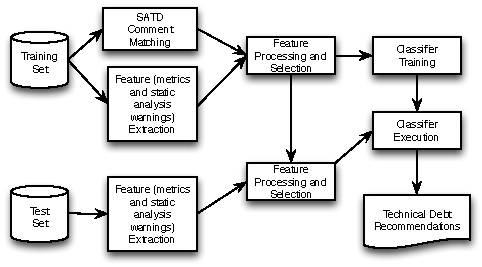
\includegraphics[width=\linewidth]{figs/approach.pdf}
	\caption{Proposed approach for recommending SATD with TEDIOUS.}
	\label{fig:approach}
	\vspace{-4mm}
\end{figure}

\ac{TEDIOUS} works as shown in Figure \ref{fig:approach}. Two datasets are required as inputs: the training set and the test set. The training set contains labeled data, which is source code from a project where technical debts are known and have been self-admitted through comments. The test set contains unlabeled data, which can be any source code under development or already released where \ac{TEDIOUS} can attempt to recommend where \ac{TD} should be self-admitted or where source code should be improved. \par 
	
For the training set, various kinds of metrics and static analysis warnings are extracted from the source code as well as \ac{SATD} methods in order to build an oracle to train the model. These labeled \ac{SATD} methods are essential for the machine learner since supervised learning is performed, meaning each method is labeled as true (containing a TD) or false. \par 

Once all the information is extracted, feature preprocessing and selection is applied. Multi-collinearity, a phenomenon occurring when two predictor variables are highly correlated, meaning that one can be linearly predicted by the other, is dealt with. Feature selection is applied to retain only the most relevant variables to train the predictor. Finally, re-balancing is performed to address the issue of the low amount of positive examples, \textit{i.e.} \ac{SATD} methods. With the preprocessed features and the oracle now defined (each method is labeled as \ac{SATD} or not), the machine learners can be trained. \par 

In parallel, the test set is also being prepared. The same features are extracted from the source code but no \ac{SATD} matching is required since the data is unlabeled. \ac{SATD} are only required for the oracle, which is used for training the models. A similar feature filtering is applied, except for the re-balancing since it is only required on the labeled data. With both the test set and the previously trained classifier, predictions can be made on the test set in order to recommend when to self-admit technical debts. \par

Each step of the process will be described in the following sections. Firstly, the features used in more details: source code metrics and warnings raised by static analysis tools. Secondly, the method employed to identify \ac{SATD}. Thirdly, the feature preprocessing: multi-collinearity, feature selection and re-balancing. Finally, the training and application of the machine learning models.

\subsection{Features}

%3 pages

Three pieces of information extracted from the source code are necessary to accurately describe the source code: structural metrics, readability metrics and warnings raised by static analysis tools. There are reasons these specific characteristics were retained to describe the source code. The structural metrics are essential to capture symptoms of complex, heavily couples and poorly designed code. These metrics explain the quality of the implementation and the software's design. The readability metrics quantify symptoms of poorly documented code or hard to read and understand. Warnings from static analysis tools are related to more specific bad choices rather than globally bad code. They are issues which could lead to low maintainability and understandability of the code or which could potentially introduce defects in the future. In the following sections, these metrics and warnings are described more in depth.

\subsubsection{Source Code Metrics}

Source code metrics are extracted to characterize its size, coupling, complexity and number of comments for readability. Nine source code metrics are used. To define the size, metrics like \ac{LOC} or number of statements are calculated. For coupling, a metric such as number of call sites is computed. For complexity, McCabe cyclomatic complexity \citep{mccabe1990reverse}, number of defined variables, number of expressions and number of identifiers are calculated. It is important to know that not all comments are considered. \ac{SATD} related comments are ignored in the empirical evaluation to avoid \ac{TEDIOUS} becoming a self-prophecy. This issue will be covered later in the study design. \par

Firstly, to extract those source code metrics, an XML representation of the Java source code was generated using the srcML tool \citep{CollardKM03} and metrics' computation was applied to it. It was also required to link comments to their related methods. The rule used was that any comments directly preceding or inside a method was assigned to it, rather it be a block of comments or just a single line. This step is essential to be able to classify which method is a \ac{SATD} and which one is not. Some methods were excluded from our analysis because they did not fit the context of our research, namely getter and setter methods since they are irrelevant with design debts. To do so, we looked for method prefixes matching \emph{get} or \emph{set} and made up from at least a single line of code. When these two criteria were covered, the method was removed from the dataset. \par 

%Using  the {\em  srcML} tool, we processed each Java file, and stored the XML Java representation. We then used the Python ElementTree XML package to build the file level document object model; visiting the DOM and extracting methods along with  the attached comments and computing a set of structural metrics \Foutse{are these metrics different from those described in the approach section?}. We assigned to a method the method proceeding comments not separated from the method definition by any other statement. Then, as also described in Section \ref{sec:approach}, for each method we extracted source code structural metrics, the Buse and Weimer readability metric, and then we executed CheckStyle and PMD on each source code file. Finally, we mapped CheckStyle and PMD warnings onto methods, by knowing the line(s) in which a warning occurred and the line span of each method.

Secondly, to extract the code readability metric, we use the one proposed by \citet{Buse:tse2010} and its related tool, based on a machine learning approach. This metric is based on specific characteristics of the source code: indentation, line length, identifier length, comment density, and the use of keywords and operators. The tool was also designed using feedback from human annotators, they were asked to rate the readability of code snippets, that was then used to classify snippets as "less" or "more" readable. A value between 0 and 1 is then computed based on these characteristics, 1 being the highest readability. The readability metric was considered relevant because, as mentioned by \citet{BavotaR16}, code readability is strongly correlated with the introduction of technical debts. Source code that is difficult to read is consequently difficult to maintain and understand \citep{Buse:tse2010} thus more likely to contain \ac{TD}. Finally, here are the nine source-code metrics we extracted: \par

\begin{itemize}
\item \textit{LOC}: Number of lines of code in the body of a method. % (excluding comments).
\item \textit{Number of statements}: Number of occurrences of expression statements in a method. In case of local class definitions, the number of statements in the enclosing method is increased by the total number of statements of the local class.
\item \textit{Number of comments}: Number of single-line and multi-line comments in a method.
\item \textit{McCabe cyclomatic complexity}: Number of linearly independent paths of a method \citep{mccabe90}.
\item \textit{Number of passed parameters}: Number of parameters of a method.
\item \textit{Number of identifiers}: Number of unique identifiers in a method.
\item \textit{Number of call sites}: Number of locations in the code where zero or more arguments are passed to a method, or zero or more return values are received from the method.
\item \textit{Number of declarations}: Number of variable and class declaration in a method.
\item \textit{Number of expressions}: Number of expressions contained in a method.
\end{itemize}

\subsubsection{Warnings Raised by Static Analysis Tools}

Warnings raised by static analysis tools are essential to detect poor coding practices, which are also related to the introduction of technical debts. We cannot directly relate a single flagged practice to a \ac{TD}. However, we can wonder if several flags are justifiable or not, and if they can be caused by the presence of a \ac{TD} in the source code. Having this hypothesis in mind, we used two popular static analysis tools, namely CheckStyle and PMD. Firstly, CheckStyle \citep{checkstyle} is widely used to check the adherence to coding standards and pieces of code that are potentially smells. It performs its analysis based on a configuration file, which can be modified at the discretion of the users. For our research, the default configuration containing code styles defined by Oracle and 43 checks was used. PMD \citep{pmd} main goal is to find common programming flaws such as unused objects, unnecessary catch blocks or incomprehensible naming. Similarly to CheckStyle, the default configuration was used, which contains 168 checks. Several reasons explains the choice of these two static analysis tools: they are adopted by \ac{OSS} \citep{BellerBMZ16}, they provide a wide range of warnings related to code styles and programming practices and they can be executed on source code statically. It is important to know that \ac{SATD} comments were removed when performing the analysis.

\subsection{Identification of Self-Admitted Technical Debt}

%0.5 page

As mentioned previously, the purpose of this thesis is not to propose a novel approach to detect \ac{SATD} using information from comments. Previous work has been completed aiming to address this issue by using  matching \citep{MaldonadoS15}, \citep{PotdarS14} or \ac{NLP} combined with machine learners \citep{maldonado17}. However, we still needed a dataset with methods tagged as design debt to train our machine learning models. \citet{maldonado17}, which worked on the \ac{NLP} approach, published a dataset of 10 open source projects annotated with methods tagged as technical debt or not. We used this dataset for our machine learning models and only the design debts were retained. \par

Some preprocessing had to be done on the dataset since it reported \ac{SATD} at file-level and not method-level. To link \ac{SATD} to methods, we matched the \ac{SATD} comment string to the comments attached to methods. We used pattern matching in order to achieve this result, making sure that method comment strings completely matched \ac{SATD} comments before tagging it as a technical debt.

\subsection{Feature Preprocessing}

%3 pages

Several characteristics have been extracted from the source code, however, not all of them are relevant or necessary to train our models. Some clean up have to be done to reduce the size of the data input and improve the training phase. Multi-collinearity have to be dealt with, feature selection as to be applied as well as training set re-balancing.

\subsubsection{Multi-Collinearity}

We computed several features to characterize the source code of the projects, however, some of them can be strongly correlated and vary in the same way. Keeping these pairs of features would cause redundancy since they can be mutually linearly predicted. That is why, when facing a pair of such features, we only keep the one that better correlates with the dependent variable, the \ac{SATD} methods. The \emph{varclus} function in R, from the \emph{Hmisc} package, was used to help us achieve this preprocessing. This function performs a hierarchical cluster analysis of features to detect when two variable are positive based on similarity measures. It is mainly used to assess collinearity and redundancy, consequently resulting in data reduction. Hoeffding D statistic, squared Pearson or Spearman correlations measures can be applied. In this research, the Spearman's $\rho$ rank correlation measure was retained. To identify the problematic duos, the cluster tree has to be cut at a particular level of $\rho^2$, which represents the correlation value. In our case, a value of $\rho^2=0.64$ was used since it corresponds to a strong correlation \citep{Cohen-1988}.

\subsubsection{Feature Selection and Normalization}

Some features will vary a lot or not at all between methods. These features are not useful to build a predictor because they can't be used as proper learning variables, they won't be determinant compared to all the other features. The process of selecting only a relevant subset of all possible features is called feature selection. Several reasons can justify going through this selection: improving the prediction performance of machine learning models, improve the speed and cost-effectiveness of predictors, and simplify the models to better understand and interpret the underlying process behind the dataset generation \citep{guyon2003introduction}. \par 

The \emph{RemoveUseless} filter implemented in Weka \citep{hall2009weka} was used to perform feature selection. It looks for features that never vary or features that vary too much. For the latter, it looked for features that had a percentage of variance above a specific treshold, which was set to 99\%. \par 

In addition to feature selection, the metrics were also normalized. Several projects were analyzed, all having significant differences in complexity and size characteristics. Those aspects of the dataset will be covered in the study definition section. This normalization is necessary to reduce the effect of those differences on the predictor's training and to achieve good cross-project prediction performance.

\subsubsection{Re-Balancing}

To build performing predictors, a quality training set must be fed to the machine learner. One important aspect is to have a balanced dataset, which means having as much as possible an equal number of positive and negative examples, in our context, as many \ac{SATD} tagged methods as clean methods. This is a serious problem in our dataset since the vast majority of methods are not technical debts (this will be discussed more in depth in the next section), only a minority contain \ac{SATD}. There are two ways to address this issue: under-sample the majority class (methods with no \ac{SATD}) or over-sample the minority class (\ac{SATD} tagged methods). Since the training set is so highly unbalanced, the number of instances of the minority class is excessively small, the second option was favored. In fact, under-sampling would result in a very small training set. To apply over-sampling, artificial instances of \ac{SATD} methods must be generated from the existing ones. To do so, Weka provides a tool to perform over-sampling, called\ac{SMOTE} \citep{chawla2002smote}, which combines under-sampling the majority class and over-sampling the minority class to achieve improved classifier performance.

\subsection{Building and Applying Machine Learning Models}

%0.5 page
 We extracted various metrics, we identified \ac{SATD} methods and we performed a preprocessing on features, the only remaining step is building and applying the machine learning models. Two sets are required: the training set and testing set. The training set contains the methods with their corresponding features and an additional variable to tag them as positive or negative (\ac{SATD} or not). It is used to build the models. The testing set contains the same methods with the corresponding features, but not the variable tagging the methods because we want to test the prediction performance from a blank dataset. We experimented with five types of machine learners in Weka \citep{hall2009weka}: Decision Trees (J48), Bayesian classifiers, Random Forests, Random Trees, and Bagging with Decision Trees. Only the default configurations were used, however, further work could be made by trying to optimize these configurations. Here is a little overview of each algorithms: \par 

\begin{itemize}
\item \textit{Decision trees}, namely J48, which implements the standard C4.5 algorithm using the concept of information entropy \citep{Quinlan1993}.
\item \textit{Bayesian classifiers}, which apply the Bayes' theorem to classify observations, assuming strong independence between features. More specifically, we use BayesNet in Weka, which is the base class for Bayes Network classifiers. It provides datastructures and facilities common to learning algorithms K2 and B.
\item \textit{Random forests}, which averages multiple decision trees trained on different parts of a same training set, with the aim to reduce the variance of the classifications and the risk of overfitting to the training set \citep{Breiman2001}.
\item \textit{Random trees}, which build decision trees considering a number of randomly chosen attributes at each node.
\item \textit{Bagging}, which combines multiple classifiers (decision trees in our case) built on random samples of the training set \citep{Breiman1996}. It was designed to improve the stability and accuracy of machine learning algorithms, to reduce the variance and to avoid overfitting.
\end{itemize}

 
\begin{landscape}
 \begin{figure}[t]
 	\centering
 	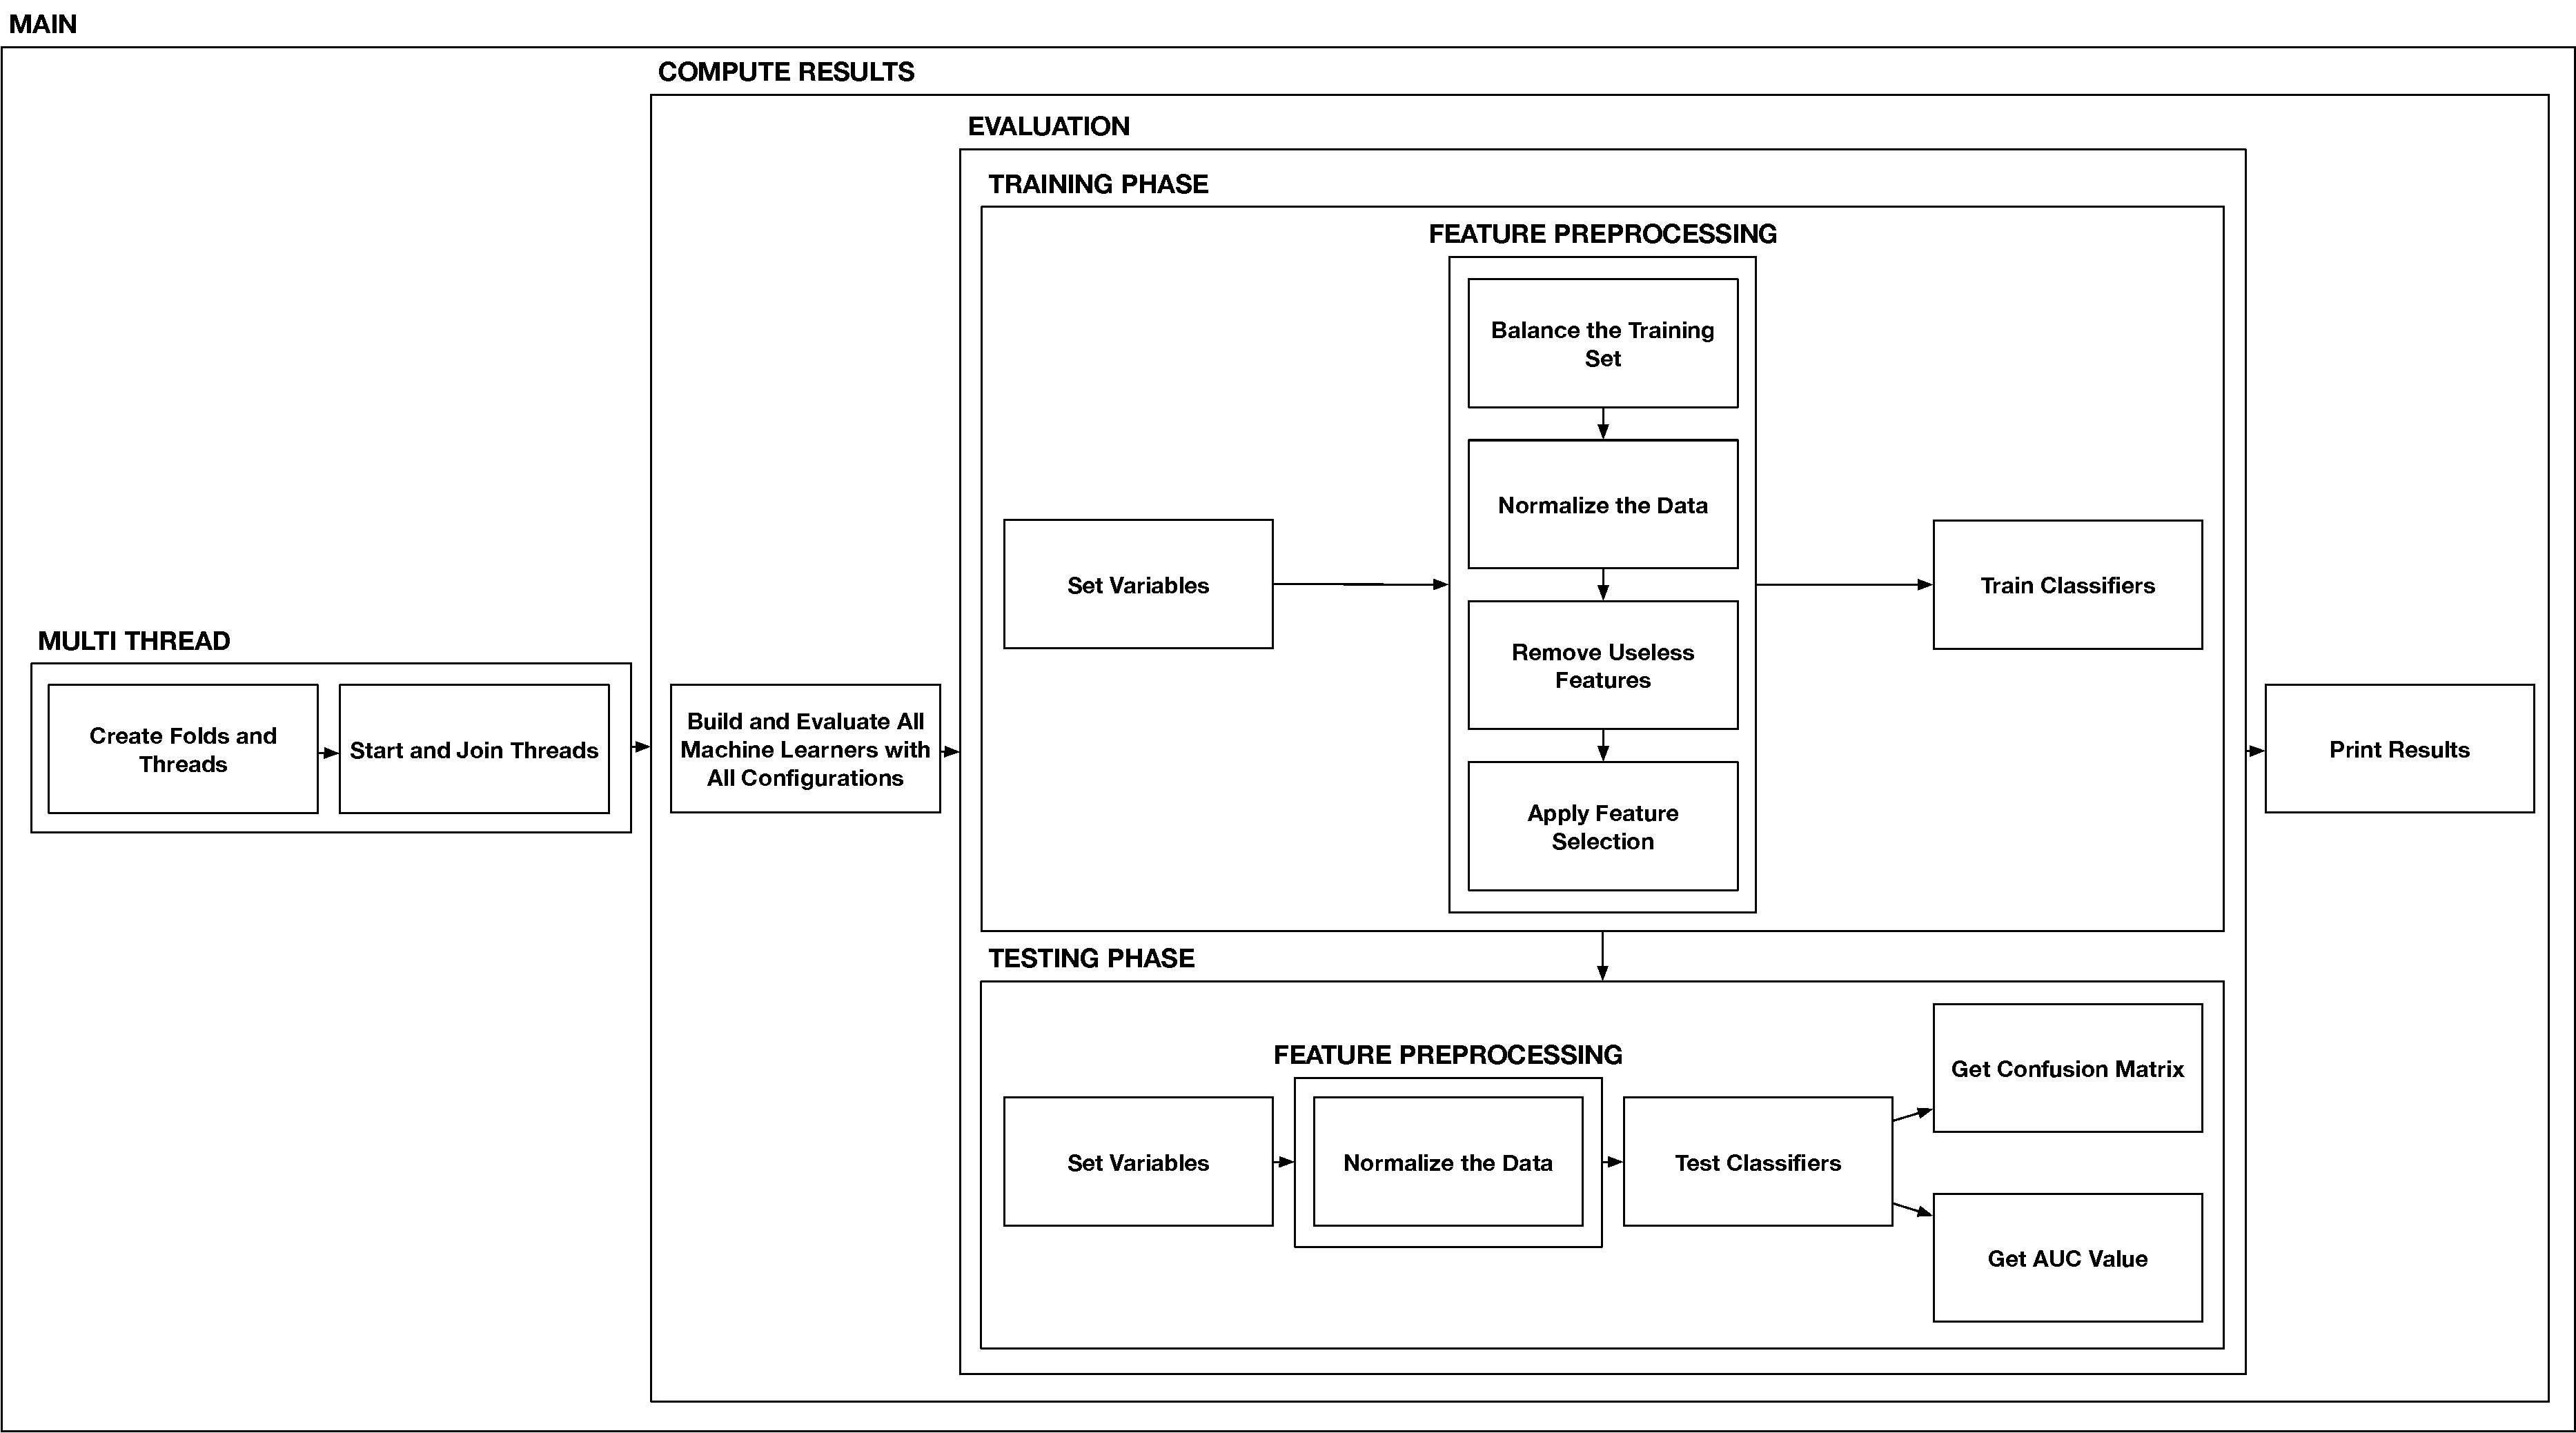
\includegraphics[width=\linewidth]{figs/MachineLearning.pdf}
 	\caption{Process for building and applying machine learners.}
 	\label{fig:MLProcess}
 	\vspace{-4mm}
 \end{figure}
\end{landscape}
 
 %\textbf{SHOW IMAGE OF PSEUDOCODE AND EXPLAIN IT. VOIR LE ECLIPSE PROJECT QUE FIORELLA A ENVOYE.} 
 
 Figure \ref{fig:MLProcess} provides an overview of the machine learning process. To increase its speed, several threads are created. For the 10 fold cross-validation inter-project analysis, one thread is started for each fold, which were generated beforehand for each software system. The following actions are performed simultaneously on each thread and the computation is finished once each of them are finished. All possible combinations of machine learners and configurations are trained and tested on each fold. We have 5 different types of machine learners, the possibility of balancing the training set or not, and the possibility of applying feature selection or not, for a total of 20 predictors. \par
 
 The evaluation step consists of a training and testing phase. In the training phase, the variables to predict are set, \emph{i.e} \ac{SATD} methods, and feature preprocessing is applied. The training set can be balanced or not, data is normalized, useless features are removed and feature selection is applied or not. The models can then be trained. In the testing phase, the variables to predict are set again, as for the feature preprocessing, only data normalization is performed. The classifiers are tested and then the confusion matrix and the AUC value computed. Results are finally printed to perform further analysis.
 
\section{Study Definition}

%0.5 page

The goal of this thesis is to assess the prediction performance of our machine learning based approach in recommending technical debts to self-admit. The focus is to enhance source code quality, more specifically its maintainability and understandability, by keeping track of technical debts which can be corrected in the future. The perspective of this thesis is to be able to suggest to developers when to admit technical debts. We aim at addressing three research questions:

\begin{itemize}
	\item \textbf{RQ1}: How does \ac{TEDIOUS} work for recommending \ac{SATD} within-project?
	\item \textbf{RQ2}: How does \ac{TEDIOUS} work for recommending \ac{SATD} across-project?
	\item \textbf{RQ3}: How would a method-level smell detector compare with \ac{TEDIOUS}?
\end{itemize}

\subsection{Dataset}

%2 pages

\begin{landscape}
\begin{table*}[t]
	\caption{Characteristics of the studied projects.}
	\label{tab:projects}
	\centering
		\begin{adjustbox}{center}
			\begin{tabular}{l r | r r r r | r | r r | r}
				\hline
				\multirow{2}{*}{Project} & \multirow{2}{*}{Release} &\multicolumn{4}{c|}{Number of} &\multicolumn{1}{c|}{Number of Comments}
				&\multicolumn{2}{c|}{Number of Design SATD} & \% of Methods\\
				&& Files& Classes& Methods& Comments                      & $\in$ Methods& $\notin$ Methods & $\in$ Methods & with design SATD\\
				\hline
				Ant&1.7.0 & 1,113 & 1,575 & 11,052 & 20,325               & 13,359        &  1 & 57 & 0.5\% \\
				ArgoUML&0.34& 1,922 & 2,579 & 14,346 & 64,393       &  17,722       & 203 & 425  & 2\%\\
				Columba&1.4& 1,549 & 1,884 & 7,035 & 33,415           & 10,305        & 8 & 418 & 5\%  \\
				Hibernate&3.3.2 GA & 2,129 & 2,529 & 17,405 & 15,901 & 9,073        & 21  &  377  &  2\%\\
				jEdit & 4.2 & 394 & 889 & 4,785 & 15,468                     &10,894         & 6  & 77  & 2\% \\
				jFreeChart&1.0.19 & 1,017 & 1,091 & 10,343 & 22,827  & 15,412       &  4  & 1,881  & 18\%\\
				jMeter&2.1& 1,048 & 1,328 & 8,680 & 19,721                &  12,672      & 95 &  424 & 5\%  \\
				jRuby&1.4.0 & 970 & 2,063 & 14,163 & 10,599               & 7,809        & 16   & 275  &  2\%\\
				Squirrel&3.0.3 & 2,325 & 4,123 & 16,648 & 25,216         & 15,574      &35  & 173  & 1\%\\
				\hline
			\end{tabular}
		\end{adjustbox}
		\vspace{-4mm}
\end{table*}
\end{landscape}

To evaluate our approach, we used a dataset that was already analyzed to find \ac{SATD} methods \citep{maldonado17}. It consists of ten open source projects, although we used only nine of them since we could not download the specific version of EMF, where \ac{SATD} were detected using a \ac{NLP} approach. The methods were then manually validated and classified. Table \ref{tab:projects} summarizes the characteristics of all studied projects. It provides information on project releases; number of files, classes, methods and comments in projects; number of comments in methods; number of design \ac{SATD} in methods and not in methods; and percentage of methods with design \ac{SATD}. \par

Some differences were observed with the characteristics extracted from the original paper \citep{maldonado17}, concerning the number of classes, methods and comments. Several reasons can explain these disparities: different extraction tooling, tools characteristics and processing. For example, we considered each comment as a single entity, whereas \citet{maldonado17} regrouped successive line comments. Additionally, we did not establish a separation between classes and their inner classes, and we considered interfaces as classes. Methods related to inner classes were associated to its container. However, these differences are not an issue for our research since they concern classes and our approach is method-level based. Some files from \citet{maldonado17} analysis could have been left aside because of their absence of comments. \par 

We can obtain some interesting information when looking at Table \ref{tab:projects}. As explained previously, we clearly see a prevalence of method-related \ac{SATD} compared to class-level \ac{SATD}. They are at least 2 times more common for \textsc{ArgoUML}, which contains about half of all the class-level \ac{TD} in the dataset, and can be up to 470 times more common for \textsc{jFreeChart}, only 4 out of the 1,885 design \ac{SATD} are at class-level. Globally, we are around 10 times more likely to encounter a method-level design technical debt in our dataset than class-level. We also observe that the dataset is highly unbalanced between \ac{SATD} prone and non \ac{SATD} prone methods. \textsc{jFreeChart} provides a decent ratio with 18\% of methods containing a design \ac{TD} but all other projects have 5\% or less of their methods containing design debts. To put this into perspective, out of the 11,052 methods in \textsc{Ant}, only 57 are \ac{SATD} prone. For \textsc{jEdit}, only 77 instances out of 4,785 are proned to contain a \ac{SATD}. Unsurprisingly, as we will discuss in the analysis of study results, these two projects achieved the lowest performance values. \par 

The replication package provided by \citet{maldonado17} contains information on \ac{SATD} at class-level. However, to build the oracle, we need to assign \ac{SATD} at method-level. To do so, we performed pattern matching between known \ac{SATD} comments and comments attached to methods. If a comment is matched inside a class but not a method, it is attached to the class, if it is matched outside of a class, it is attached to the file. These class-level and file-level technical debts are not considered in our research, which is not a big issue since they represent the minority.

\subsection{Analysis Method}

%3.5 pages

For \textbf{RQ1}, we want to know how \ac{TEDIOUS} works for recommending \ac{SATD} within-project. A 10-fold cross validation was performed on each project. In other terms, the dataset of a single project is divided into 10 folds, the machine learner is trained on 9 of them and tested on the remaining one, until all 10 configurations are processed to limit the effect of randomness. The performance values are averaged over the 10 iterations to obtain the most representative picture. For \textbf{RQ2}, we want to know how our approach works for recommending \ac{SATD} across-project. The process is similar to \textbf{RQ1}, but instead we train on 8 projects and test on the remaining one, until all the 9 possible combinations are executed. \par 

Standard performance metrics for evaluating automated classification were computed to analyze our approach: precision, recall and $F_{1}$ score. These metrics were computed for the \ac{SATD} category. \par 

\ac{Pr} is the percentage of relevant instances of methods predicted as \ac{SATD} among all retrieved instances. \ac{TP} and \ac{FP} are the number of true positives, correct methods predicted as \ac{SATD}, and false positives, incorrect methods predicted as \ac{SATD}.

\[
Pr=\frac{TP}{TP+FP}
\]

\ac{Rc} is the percentage of relevant instances of \ac{SATD} methods that have been retrieved over all relevant instances. \ac{FN} is the number of false negatives, incorrect methods predicted as non \ac{SATD}.

\[
Rc=\frac{TP}{TP+FN}
\]

The $F_{1}$ score is the harmonic mean between precision and recall, which provides a single measurement for evaluating a system.

\[
F_1=2 \cdot \frac{PR \cdot RC}{PR + RC}
\]

The previous metrics are specific to the \ac{SATD} class, which means true negatives \ac{TN}, correct methods predicted as non \ac{SATD}, are not considered. Consequently, other metrics are required to complement the analysis: accuracy, Matthews Correlation Coefficient (MCC) \citep{matthews1975comparison}, and the Area under the Receiving Operating Characteristics (ROC) Curve (AUC). \par 

\ac{Acc} is the total number of methods correctly predicted, whether it is containing a \ac{SATD} or not, among all the methods analyzed.

\[
Acc=\frac{TP+TN}{TP+TN+FP+FN}
\]

The \ac{MCC} is a metric used in machine learning to evaluate the quality of a two-class classifier. It is especially useful when the dataset is unbalanced \citep{matthews1975comparison}. Values vary between -1 for a completely wrong classifier and 1 for a completely correct classifier. 

\[
MCC=\frac{TP \cdot TN-FP \cdot FN}{\sqrt{(TP+FP)(FN+TN)(FP+TN)(TP+FN)}}
\]

The \ac{ROC} curve is created by plotting the true positive rate against the false positive rate at various classifier thresholds. The \ac{AUC} is the area under the ROC curve, it provides a value to evaluate the quality of the classifier. A value of AUC=0.5 refers to a random classifier and the higher the value, the better the classifier.

To have a good idea of the performance of each machine learner, each of the previous metrics have to be considered in the evaluation. We want a balance between precision and recall because we want as much as possible to detect real technical debts and all of them. We cannot only use $F_{1}$ score because we want to take into account the effect of chance on the predictions. Thats is why we also computed the MCC and AUC values.

In addition to these performance indicators, we also consider the importance of each features for the training of the predictors. We used a technique implemented in Weka for Random Forests named \ac{MDI} \citep{louppe2013understanding}, which measures the importance of variables on randomized decision trees.

For \textbf{RQ3}, we want to compare \ac{TEDIOUS} with a popular method-level smell detector (DECOR) \citep{moha2010decor} in classifying as technical debt methods labeled as \ac{SATD}. DECOR can detect a large amount of smells, but most of them are at class-level, which are not relevant with the level at which \ac{TEDIOUS} works. Instead of using all of them, we narrowed our analysis on two method-level smells, \textit{Long Method} and \textit{Long Parameter List}. To identify a Long Method smell, DECOR follows the rule {\em LOC}$>th_1$ where $>th_1$ is a threshold for the LOC. To identify a Long Parameter List smell, DECOR follows the rule {\em ParNbr}$>th_2$ where {\em ParNbr}$>th_2$ is a threshold for the number of parameters. Various thresholds for LOC and ParNbr were considered in our research, between percentile 0.5 and 0.95, as well as the default thresholds, namely percentile 0.75 for LOC and outlier (third quartile $+ 1.5 \cdot IQR$ (interquartile range)) for ParNbr.

To finish, we performed a qualitative analysis on false positives and false negatives examples we obtained when evaluating our predictors. Its purpose is to complement our quantitative analysis and discuss the limitations of our approach in recommending \ac{TD} with real examples.
























             % Premier thème (Doctorat) ou "Détails de la Solution" (Maîtrise).
\Chapter{ANALYSIS OF STUDY RESULTS AND THREATS TO VALIDITY}\label{sec:Theme2}

%TOTAL = 18 pages

\section{Study Results}

This section reports the study results in the context of each research question. Tables provide visual representation and summarize the main results. More in depth analysis is discussed for the three research questions and the qualitative analysis.

\subsection{How does TEDIOUS work for recommending SATD within-project?}

%4.5 pages

\begin{table}[t]
	\caption{Average performance of different machine learners for within-project prediction.}
	\label{tab:avgWithin}
	\centering
	\resizebox{\linewidth}{!}{
		\begin{tabular}{lrrrrrr}
			\multicolumn{7}{c}{ \textbf{Without Balancing}}\\
			\hline
			\textbf{ML} & \textbf{Pr} & \textbf{Rc} & \textbf{F$_{1}$} &\textbf{Acc} &\textbf{MCC} &\textbf{AUC}\\
			\hline
			\rowcolor{grey}
			\textbf{Random Forests} &49.97 &52.19&47.15&93.32&0.47&0.92\\
			\textbf{Bagging} &51.91 &48.45	&45.97&93.35&0.45&0.92\\
			\textbf{Bayesian} & 24.29&78.77&34.18&89.01&0.38&0.93\\
			\textbf{j48} & 34.86&54.42&39.54&94.18&0.39&0.82\\
			\textbf{Random Trees} &23.09&52.49&29.96&90.35&0.30&0.73\\
			\multicolumn{7}{c}{\textbf{With Balancing}}\\
			\hline
			\textbf{ML} & \textbf{Pr} & \textbf{Rc} & \textbf{F$_{1}$} &\textbf{Acc} &\textbf{MCC} &\textbf{AUC}\\
			\hline
			\rowcolor{grey}
			\textbf{Random Forests} & 26.56&68.26&36.04&90.45&0.37&0.92\\
			\textbf{Bagging} & 18.4&75.12&28.24&85.58&0.31&0.90\\
			\textbf{Bayesian} & 4.00&94.07&7.55&15.66&0.04&0.72\\
			\textbf{j48} & 16.95&77.76&26.45&84.04&0.30&0.85\\
			\textbf{Random Trees} &16.03&63.22&24.49&85.34&0.26&0.75\\
			\hline
	\end{tabular}}
	\vspace{-3mm}
\end{table}

Table \ref{tab:avgWithin} presents the average performance results of a 10-fold cross validation within-project executed 10 times and on different machine learners. The average was computed for the 9 studied projects. The 10-fold cross validation was performed with balancing using SMOTE and without balancing.

On the unbalanced dataset, the best classifier is the one using the Random Forests algorithm. It achieves the best balance between precision ($49.97\%$) and recall ($52.19\%$), obtaining a $F_{1}$ score of $47.15\%$, the highest of all machine learners. We also notice that the Bagging algorithm is performing almost as well as Random Forests, even obtaining a slightly better precision but a weaker $F_{1}$ score. The accuracy of Random Forests, which includes the correct classification of negatives (the vast majority of the data), is $93.32\%$ and almost all the other machine learners obtain an accuracy higher than $90\%$, between $[89.01\%-93.35\%]$. MCC is on average $>0.4$, which is translated into a moderate correlation, and AUC is $>0.9$ (close to a perfect classifier) for Random Forests, Bagging and Bayesian and $>0.7$ for j48 and Random Trees.

On the balanced dataset, the best classifier is still Random Forests, with a precision of $26.56\%$, recall of $68.26\%$ and $F_{1}$ score of $36.04\%$. Its MCC value is the highest at $0.37$, moderate correlation, and the same goes for its AUC value which is the same as previously, $0.92$. The purpose of balancing is achieved since the recall of each machine learners is higher than previously, at the expense of precision. There is a clear gap between the Bayesian classifier and the others, it is definitely performing more poorly. All the performance values are the worst, except for the recall which is really good but not enough to compensate. In fact, it performs like a random classifier if we look at the MCC value which is almost $0$. The other classifiers all performed similarly, having a precision between $[16.03\%-18.40\%]$, a recall between $[63.22\%-75.12\%]$ and a $F_{1}$ score around $25\%$. Their MCC value is around $0.3$, which translates to a fair correlation and the AUC value is decent at $0.7$ or more. However, the results are globally weaker with balancing than without it.

\begin{table}[t]
	\caption{Within-project prediction: results of Random Forests for each system, without and with SMOTE balancing.}
	\label{tab:bysyswithin}
	\centering\scriptsize
	\resizebox{\linewidth}{!}{
		
		\begin{tabular}{lrrrrrr}
			%\hline
			\multicolumn{7}{c}{ \textbf{Without Balancing}}\\
			\hline
			\textbf{System} & \textbf{Pr} & \textbf{Rc }&\textbf{F$_{1}$} &\textbf{Acc} &\textbf{MCC} &\textbf{AUC}\\
			\hline
			Ant &0.91& 16.39 & 1.73 & 84.59 & 0.00 & 0.77\\
			ArgoUML &85.19& 38.10 & 52.65 & 93.25 & 0.54&0.91\\
			Columba & 36.40 & 65.94 & 46.91 & 96.02 & 0.47 & 0.94\\
			Hibernate & 53.44 & 65.22 & 58.74 & 96.80 & 0.57 & 0.97\\
			jEdit & 5.24 & 25.71 & 8.71 & 85.51 & 0.06 & 0.81\\
			jFreeChart & 84.58 & 82.52 & 83.54 & 98.91 & 0.83 & 0.99\\
			jMeter & 53.38 & 47.37 & 52.30 & 96.69 & 0.51 & 0.94\\
			jRuby & 52.27 & 84.02 & 64.45 & 94.21 & 0.64 & 0.97\\
			Squirrel & 73.33 & 44.44 & 55.35 & 99.51 & 0.57 & 0.97\\
			\multicolumn{7}{c}{ \textbf{With Balancing}}\\
			\hline
			\textbf{System} & \textbf{Pr} & \textbf{Rc }&\textbf{F$_{1}$} &\textbf{Acc} &\textbf{MCC} &\textbf{AUC}\\
			\hline
			Ant & 2.46& 44.26 & 4.67 & 85.02 & 0.08 & 0.83\\
			ArgoUML &47.03 & 65.39 & 54.71 & 89.34 & 0.50&0.90\\
			Columba & 15.35 & 74.64 & 25.46 & 88.35 & 0.30 & 0.94\\
			Hibernate & 19.85 & 89.13 & 32.47 & 87.04 & 0.38 & 0.95\\
			jEdit & 7.74 & 34.29 & 12.63 & 87.25 & 0.11 & 0.86\\
			jFreeChart & 62.98 & 92.68 & 75.00 & 97.94 & 0.75 & 0.99\\
			jMeter & 32.03 & 64.47 & 42.79 & 93.40 & 0.42 & 0.92\\
			jRuby & 32.75 & 91.91 & 48.29 & 87.72 & 0.50 & 0.92\\
			Squirrel & 18.81 & 57.58 & 28.36 & 98.02 & 0.32 & 0.96\\
			\hline
		\end{tabular}
	}
	\vspace{-3mm}
\end{table}

Table \ref{tab:bysyswithin} highlights the within-project prediction results, for each system, using Random Forests, and using balancing or not. Random Forests only was used since it is best classifier based on Table \ref{tab:avgWithin}. If we look at the unbalanced dataset, two systems are performing way worse than the others, namely \textsc{Ant} and \textsc{jEdit}. There is a reason behind this if we look back at Table 3.1. The projects, other than \textsc{jFreeChart} with 18\%, all have a percentage of their methods containing SATD below or equal to 5\%. \textsc{Ant} only has 0.5\% of its methods containing SATD and \textsc{jEdit} 2\%. This explains the low performance values of \textsc{Ant} (precision $0.91\%$, recall $16.39\%$ and $F_1$ score $1.73\%$) and \textsc{jEdit} (precision $5.24\%$, recall $25.71\%$ and $F_1$ score $8.71\%$). The AUC values are still decent, respectively with $0.77$ and $0.81$, but the MCC values, respectively with $0$ and $0.06$, clearly prove us that the classifier is as good as a random one.

\textsc{jFreeChart} is the project containing the most number of SATD and is consequently the project where the classifier performs the best. It obtains high precision and recall ($84.58\%$ and  $82.52\%$) as well as high MCC and AUC ($0.83$ and $0.99$). Performance values on the other 6 projects are also promising, the $F_1$ score is almost always $>50\%$, the MCC is between $[0.47-0.64]$ which is moderate to strong correlation, and the AUC is in the interval $[0.91-0.97]$. We notice that the prediction performance of TEDIOUS is dependent on the system and not only the number of SATD it is trained on. \textsc{Squirrel} has a slightly higher percentage of SATD methods than \textsc{Ant} and slightly lower than \textsc{jEdit}, but it still performs significantly better than these two projects ($73.33\%$ precision and $44.44\%$ recall). 

If we look at the balanced dataset, the same trend is observed as in the balanced dataset but with lower performance results. Precision is generally lower except for \textsc{Ant} and \textsc{jEdit} which obtain a small improvement. These two systems should normally benefit from balancing but the data from the few SATDs is not even enough to build a decent artificial training set, leading to a negligible gain in precision. However, as expected with balancing, we see a decent increase in their recall and the same goes for the other systems. Generally speaking, the accuracy, $F_1$ score, MCC and AUC is better for \textsc{Ant} and \textsc{jEdit} only, the other systems did not benefit from the balancing.

\begin{table*}[t]
	\caption{Top 10 discriminant features (within-project prediction). (M): source code metrics,  (CS): CheckStyle checks, (P): PMD checks.}
	\label{tab:top10features}
	\centering\scriptsize
	\resizebox{\linewidth}{!}{
		
			\begin{tabular}{lcccccccccc}
				Metric Name &Ant&ArgoUML&Columba&Hibernate&jEdit&jFreeChart&jMeter&jRuby&Squirrel\\
				\hline
				\rowcolor{grey}
				Readability (R)&5&1&2&1&1&1&1&1&1\\
				LOC (M)&2&2&5&2&2&3&2&3&4\\
				%\hline
				\rowcolor{grey}
				DeclNbr (M)&4&3&7&4&3&4&3&4&3\\
				ParNbr (M) &8&5&9&7&7&7&7&7&7\\
				%\hline
				%\hline
				%\hline
				\rowcolor{grey}
				ExprStmtNbr (M)&6&4&---&5&4&5&5&5&5\\
				%\hline
				McCabe (M)&10&7&---&6&6&6&6&6&6\\
				\rowcolor{grey}
				%\hline
				CommentNbr (M)&---&6&---&3&5&2&4&2&2\\
				%\hline
				LineLength (CS) &---&---&---&9&---&---&9&8&9\\
				%\hline
				\rowcolor{grey}
				LocalVariableCouldBeFinal (P) &---&---&---&10&9&---&---&9&10\\
				%\hline
				DataflowAnomalyAnalysis (P) &---&10&---&---&10&---&---&---&---\\
				%\hline
				\rowcolor{grey}
				FinalParameters (CS) &---&---&---&---&---&8&8&---&---\\
				%\hline
				MissingSwitchDefault (CS) &---&8&4&---&---&---&---&---&---\\
				\rowcolor{grey}
				%\hline
				AvoidReassigningParameters (P) &7&---&---&---&---&---&---&---&---\\
				%\hline
				CollapsibleIfStatements (P) &9&---&---&---&---&---&---&---&---\\
				%\hline
				\rowcolor{grey}
				EmptyIfStmt (P) &---&---&8&---&---&---&---&---&---\\
				%\hline
				IfStmtsMustUseBraces (P) &---&---&---&---&8&---&---&---&---\\
				%\hline
				\rowcolor{grey}
				LeftCurly (CS) &---&---&---&---&---&---&---&---&8\\
				%\hline
				LocalVariableName (CS) &---&---&1&---&---&---&---&---&---\\
				%\hline
				\rowcolor{grey}
				MethodArgumentCouldBeFinal (P) &---&---&---&---&---&---&---&10&---\\
				%\hline
				MethodLength (CS) &---&---&---&---&---&---&10&---&---\\
				%\hline
				\rowcolor{grey}
				OptimizableToArrayCall (P) &---&---&10&---&---&---&---&---&---\\
				%\hline
				ParameterNumber (CS) &---&---&---&---&---&10&---&---&---\\
				%\hline
				\rowcolor{grey}
				ParenPad (CS) &---&---&---&8&---&---&---&---&---\\
				%\hline
				ShortVariable (P) &---&---&---&---&---&9&---&---&---\\
				%\hline
				\rowcolor{grey}
				SimplifyBooleanReturns (CS) &---&9&---&---&---&---&---&---&---\\
				%\hline
				SwitchStmtsShouldHaveDefault (P) &---&---&6&---&---&---&---&---&---\\
				%\hline
				\rowcolor{grey}
				UselessParentheses (P) &3&---&---&---&---&---&---&---&---\\
				%\hline
				UseLocaleWithCaseConversions (P) &---&---&3&---&---&---&---&---&---\\
				%\hline
				\rowcolor{grey}
				UseStringBufferForStringAppends (P) &1&---&---&---&---&---&---&---&---\\
				%\hline
				%UseConcurrentHashMap&---&1&---&---&---&---&---&---&---\\
				%\hline
				%\rowcolor{grey}
				%UseObjectForClearerAPI&---&---&---&---&---&---&---&---&2\\
				%\hline
				%UseStringBufferForStringAppends&---&---&---&---&---&---&---&1&---\\
				%\hline
				%\rowcolor{grey}
				%WhitespaceAfter&---&---&10&---&---&---&---&---&---\\
				\hline
			\end{tabular}

	}
	\vspace{-2mm}
\end{table*}

Table \ref{tab:top10features} reports the top 10 features in within-project prediction according to the MDI technique.

\subsection{How does TEDIOUS work for recommending SATD across-project?}

4 pages

\subsection{How would a method-level smell detector compare with TEDIOUS?}

1.5 pages

\subsection{Qualitative discussion of false positive and false negatives}

4 pages

\section{Threats to Validity}

\subsection{Construct validity}

1 page

\subsection{Internal validity}

1 page

\subsection{Conclusion validity}

1 page

\subsection{External validity}

1 page

             % Second thème (Doctorat) ou "Résultats théoriques et expérimentaux" (Maîtrise).
\Chapter{CONVOLUTIONAL NEURAL NETWORK WITH COMMENTS AND SOURCE CODE}\label{sec:Theme3}

% TOTAL = 15 pages

%	./train.py --enable_word_embeddings true --num_epochs 6 --dev_sample_percentage 0.01 --positive_train=$pos --negative_train=$neg
%	
%	Used for the 3-Folds
%
% ./word2vec -train ../../tokenized-concordia-no-comment.txt -output concordia-bin-64.bin -size 100 -window 5 -sample 1e-4 -negative 5 -hs 0 -binary 1 -cbow 1 -iter 3

\section{Convolutional Neural Network}

%1 page

Several machine learners were tested with TEDIOUS, using source code metrics as training features. Results were promising but the approach asked for a lot of preparation work: building the XML representation of the Java code, pattern matching between comments from the dataset and the source code, extracting the source code metrics, extracting the warning raised by static analysis tools and feature preprocessing. These additional steps take time and knowledge of the whole process. Consequently, we wanted to try a novel approach, easier and faster to set up. We decided to test a Convolutional Neural Network (CNN) with Natural Language Processing (NLP) directly on the Java source code of software projects.

The idea of using a CNN was inspired by a paper written by \citet{kim2014convolutional}. He used a CNN for sentence-level classification tasks and showed that you can achieve excellent performance results with little parameter calibration. He tested his model on several benchmarks. Similar work has been pursued concerning sentiment analysis of short texts \citep{dos2014deep}. More specifically, they analyzed Twitter messages and movie reviews, and tried to classify them as being of positive or negative sentiment. Our idea is similar to these studies, we plan to use a CNN to classify comments and/or methods using the source code directly instead of features, linking them to technical debt or not.

Typically, convolutional neural networks were employed for image classification \citep{krizhevsky2012imagenet}, however, as mentioned previously, this type of neural network has been used recently combined with NLP. To describe CNN in further details, we can think of a convolution as a window sliding across a whole matrix, acting as a filter. For images, this matrix contains pixels, for words and sentences, it contains word vectors (word embeddings). In image classification, filters slide over local batches, in NLP, they slide over entire rows since a row is typically a single word embedded into a row matrix of the size of the embedding dimension. To implement a CNN, you just have to add several layers of these convolutions, where each of these layers have a specific task and act as different filters. CNNs are very fast and efficient in terms of representation, which means they give good representations without needing the whole vocabulary of a dataset.

The main purpose of this study was to explain, test and analysis TEDIOUS, our machine learning approach using source code features. The next sections will describe the other approach using a CNN, but at a more general level than for TEDIOUS since we are still at a preliminary stage. Since some steps from Chapter 3 are replicated in our CNN approach, they will be explained rapidly in order to avoid redundancy. However, we still judged interesting to present the initial results of this new promising method.

\section{The Approach}

%1 page

This section will describe the steps followed to design this new approach, a convolutional neural network combined with natural language processing to identify technical debts to self-admit. Additional information will be shared on the characteristics of this machine learner and how it works. Like TEDIOUS, this approach works at method-level since it is granularity at which we are most likely to detect TD \citep{PotdarS14}. In other terms, this approach is able to detect if a technical debt is contained in a method or not.

\begin{figure}[t]
	\centering
	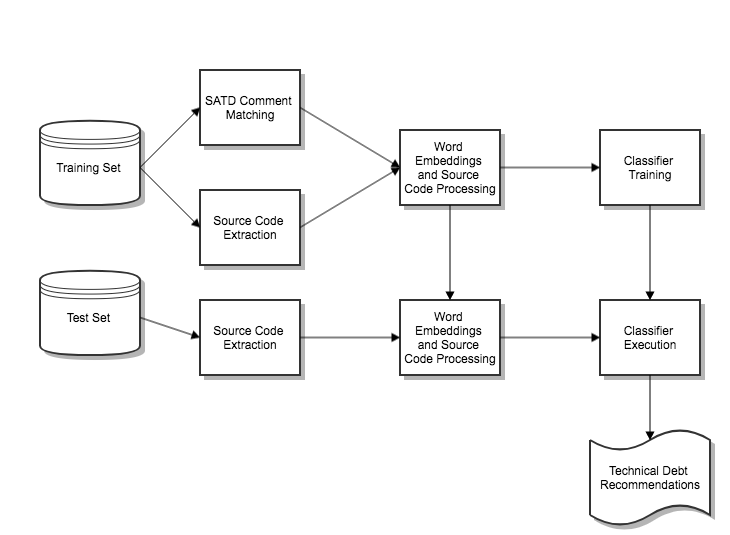
\includegraphics[width=\linewidth]{figs/CNN.png}
	\caption{Proposed approach for recommending SATD with a CNN.}
	\label{fig:CNN}
	\vspace{-4mm}
\end{figure}

As shown in Figure \ref{fig:CNN}, two datasets are required to build our model: the training and test set. The training set contains labeled data, which is source code where SATD are known. The test set contains unlabeled data, which can be any source code where we want to recommend where technical debts should be admitted. The presence and location of TDs are unknown in the test set.

For the training set, various combinations of source code and comments, labeled as containing a SATD or not, are extracted: source code comments only, source code with comments, source code without comments and source code partially with comments. It is essential to have this classification because the CNN is based on supervised learning. Pattern matching using comments from the dataset of \citet{maldonado17} is employed to classify the methods and comments.

Once all the source code is extracted and classified, some preprocessing has to be done. The source code is tokenized, the purpose being to demarcate and transform the source code into a string of word tokens. The comments specifically are cleaned up to remove extra spaces, non-ASCI characters, upper case letters, etc. Once the source code is preprocessed, word embeddings is performed, which means strings of tokens are transformed into vectors of numerical values using word2vec tool \citep{word2vec}. With the source code preprocessed and the oracle built, the model can be trained with the CNN.

In parallel, the test set is prepared. The same combinations of source code and comments are extracted, but SATD matching is not required because the data is unlabeled and we want to predict the presence of technical debts. The matching of SATDs is only required for the oracle to train models. The same preprocessing and word embeddings are applied on the dataset. With the previously trained model and the test set, predictions can be made in order to recommend when to self-admit technical debts.

An overview of the process was described in this section, but more details will be shared in the next ones. We will discuss the source code and its nature, how we identified the SATD, how we performed word embeddings and the process to train and apply the models generated by the CNN.

\subsection{Source Code}

% 1 page

The main difference between TEDIOUS and this new approach is the nature of the training features. For TEDIOUS, source code metrics and warnings were used. For the CNN, we use the source code itself, transformed into word vectors. The same process was performed as before to extract the source code, an XML representation of the Java source code was generated using the srcML tool \citep{Collard2013}. SATD comments from the dataset of \citet{MaldonadoNLP} were linked to their respective methods in order to classify them as containing a technical debt or not, to build the oracle. The same rules were followed, as explained in section 3.1.1. Once the XML representation is obtained, the different dataset combinations can be generated.

The first combination is the \textit{source code comments only}. They are extracted from the dataset of comments provided by \citet{maldonado17}. Comments can be encountered under different natures: single line, multiple lines or block. The second combination is the \textit{source code with comments} where the complete XML representation of the source code is used. The third combination is the \textit{source code without comments} where the XML representation is parsed to remove comments. The fourth combination is the \textit{source code partially with comments}, which means only comments related to SATD are removed. The reason behind this removal is to be sure to avoid the CNN model being a self-prophecy. The details of the processes will be explained in the Source Code Preprocessing section.

\subsection{Identification of Self-Admitted Technical Debt}

% 0.5 page

Like TEDIOUS, the purpose of this approach is not to propose a new way to detect SATD using information from comments. However, will still needed a classified dataset in order to train our CNN model. We used the dataset of \citet{maldonado17}, which contains a classification of 10 open source projects, where methods are tagged as containing a technical debt or not. Various types of TDs are considered, depending on the source code combination. The dataset reports SATD at file-level instead of method-level, consequently, some preprocessing had to be performed. With pattern matching, SATD comments were tagged to their related methods.

\subsection{Source Code Preprocessing and Word Embeddings}

% 1 page

The source code is extracted in a XML format, which is not quite compatible for the machine learner to train on. The files have to be tokenized. Instead of using standard coding lexicon (conditional statements, variables types and names, parameters declaration) and separators (brackets, parentheses, spaces) directly in our dataset, demarcations are added (\textit{i.e. begin\_type, end\_type}) to transform the structure into series of word tokens. For comments, strings are normalized: extra spaces are removed, upper cases are transformed to lower cases, non-ASCI are removed as well as new lines. Also, if a comment is matched with a SATD pattern, it will be printed as:

\textsc{comment\_begin\_satd    comment-normalized-text    comment\_end\_satd}

This step is essential to build the oracle and the dataset partially with comments. By explicitly defining comments tagged as SATD in this format, it is easy to parse the tokenized dataset in order to remove them. Comments are linked to their respective method, so a method linked to a SATD comment will also be tagged as SATD. By tokenizing the source code, it is also easier to remove the comments globally, if necessary. Transforming the source code into tokens also acts as a normalization process, which will make the word embedding process more efficient.

Word embeddings is the process of transforming words and phrases from the dataset into vectors of real number. Word2vec models were used to generate word embeddings. The vector dimension we used is 100, we tried to have a balance between a proper representation of words and processing time. A new word embedding was generated for each source code combination since they are all different in some ways.

Finally, the methods extracted are all tagged as positive or negative examples. In order for the CNN to be trained and tested, these methods have to be divided in 4 basic files: \textsc{positive-train}, \textsc{negative-train}, \textsc{positive-test} and \textsc{negative-train}. Each fold of the cross validation contains these 4 files, consequently, for a 10-fold cross validation, 40 files are required. Instead of using an additional feature to classify each method in a single file, the files act as classifiers. Here is a detailed definition of each file, considering a 10-fold cross validation:

\begin{itemize}
	\item \textit{Positive-Train}: Training set containing SATD methods (90\% of all positive examples)
	\item \textit{Negative-Train}: Training set containing non-SATD methods (90\% of all negative examples)
	\item \textit{Positive-Test}: Testing set containing SATD methods (10\% of all positive examples)
	\item \textit{Negative-Test}: Testing set containing non-SATD methods (10\% of all negative examples)
\end{itemize}

\subsection{Building and Applying CNN}

% 2 page

\begin{figure}[t]
	\centering
	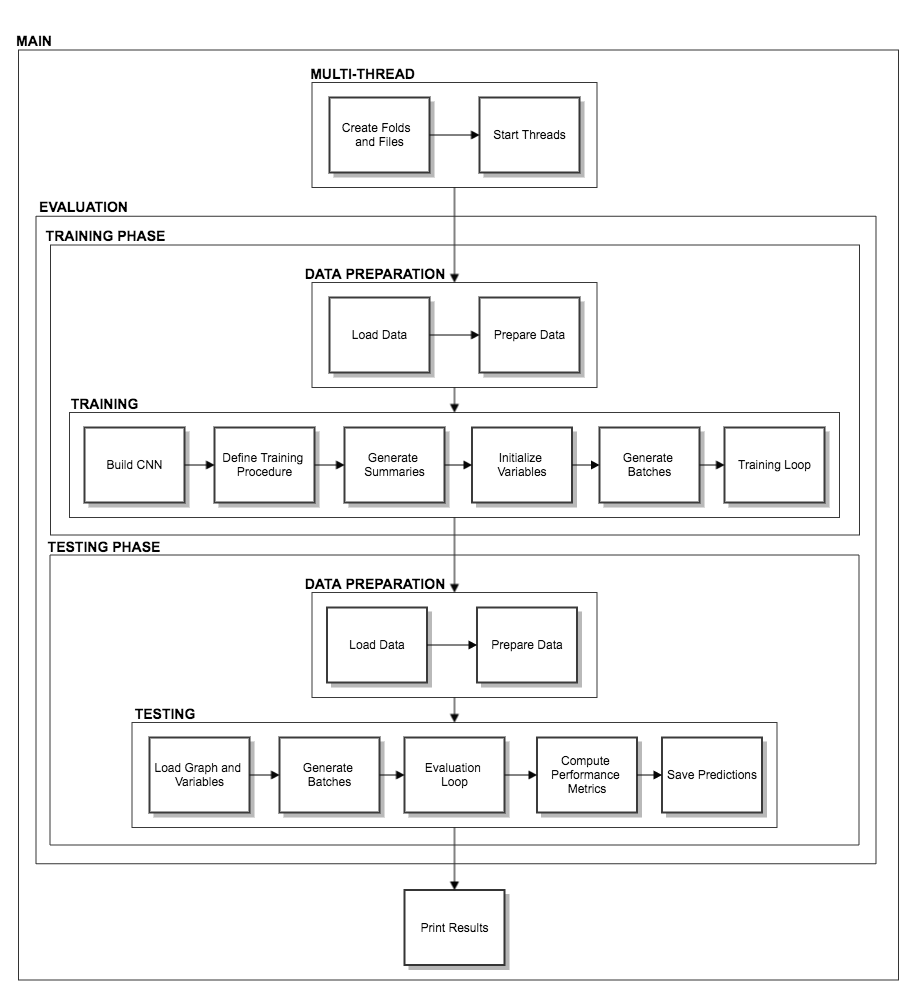
\includegraphics[width=\linewidth]{figs/CNNProcess.png}
	\caption{Process for building and applying a CNN.}
	\label{fig:CNNProcess}
	\vspace{-4mm}
\end{figure}

So far, we extracted source code from various projects, with or without comments, we identified SATD methods, we preprocessed the dataset and performed a word embedding. The only step remaining is building and applying the convolutional neural network. Four sets are required, as described in the previous section: two sets for training, one containing SATD methods and the other not, and two sets for testing, one of positive and the other of negative examples. The sets contain the tokenized source code of the nine studied projects.

Figure \ref{fig:CNNProcess} provides an overview of the CNN process. To increase the training speed and to benefit as much as possible from the processing power available, several threads are created. One thread is started for each fold, using a pair of previously generated training files. Up to five threads can be processed at the same time. The next actions are all performed simultaneously on each thread, until we have models trained for all folds. 

The evaluation process consists of two main phases: the training and the testing phase. In the former, some data preparation is required: load the two training sets, build the vocabulary, shuffle, and split the dataset in a training and development set. The development set is used to tune parameters of the CNN and to prevent it from over-fitting. Afterwards, the CNN is built using user-defined parameters and default values. In our case, mainly the default configuration is considered. The training procedure is defined and summaries are generated for: loss, accuracy, train, development and model. Then, variables are initialized, such as embedding vectors, and training batches generated. Finally, a training loop is executed where a training and evaluation step are repeated. The trained model is saved multiple times during the loop and the last one is used for the testing. 

The testing phase can start once the training is finished. Data preparation is also required for this step: load the two testing sets and map them into the vocabulary. Afterwards, the meta graph and the variables from the model previously saved are loaded. Testing batches are generated and tensors we want to evaluate are determined. We can then start the testing loop where predictions are made. Once over, performance metrics can be computed,  namely: accuracy, recall, precision, specificity and $F_1$. These metrics are saved in a different file from the predictions made on each method. The final step consists of combining the performance metrics of all models for further analysis.

\section{Study Definition}

% 0.5 page

The goal of this new approach is to assess the prediction performance of a convolutional neural network in recommending technical debts to self-admit. The focus is the same as for TEDIOUS, enhancing the source code quality by keeping track of TDs. The perspective is to be able to suggest to developers, more accurately than with TEDIOUS, when to admit technical debts. We aim to address four research questions:

\begin{itemize}
	\item \textbf{RQ1}: How does a CNN work for recommending SATD with source code comments only?
	\item \textbf{RQ2}: How does a CNN work for recommending SATD with source code  with comments?
	\item \textbf{RQ3}: How does a CNN work for recommending SATD with source code without comments?
	\item \textbf{RQ4}: How does a CNN work for recommending SATD with source code partially with comments?
\end{itemize}

\subsection{Dataset}

% 1.5 page

\begin{landscape}
	\begin{table*}[t]
		\caption{Characteristics of the studied projects.}
		\label{tab:projects}
		\centering
		\begin{adjustbox}{center}
			\begin{tabular}{l r | r r r r | r | r r | r}
				\hline
				\multirow{2}{*}{Project} & \multirow{2}{*}{Release} &\multicolumn{4}{c|}{Number of} &\multicolumn{1}{c|}{Number of Comments}
				&\multicolumn{2}{c|}{Number of Design SATD} & \% of Methods\\
				&& Files& Classes& Methods& Comments                      & $\in$ Methods& $\notin$ Methods & $\in$ Methods & with design SATD\\
				\hline
				Ant&1.7.0 & 1,113 & 1,575 & 11,052 & 20,325               & 13,359        &  1 & 57 & 0.5\% \\
				ArgoUML&0.34& 1,922 & 2,579 & 14,346 & 64,393       &  17,722       & 203 & 425  & 2\%\\
				Columba&1.4& 1,549 & 1,884 & 7,035 & 33,415           & 10,305        & 8 & 418 & 5\%  \\
				Hibernate&3.3.2 GA & 2,129 & 2,529 & 17,405 & 15,901 & 9,073        & 21  &  377  &  2\%\\
				jEdit & 4.2 & 394 & 889 & 4,785 & 15,468                     &10,894         & 6  & 77  & 2\% \\
				jFreeChart&1.0.19 & 1,017 & 1,091 & 10,343 & 22,827  & 15,412       &  4  & 1,881  & 18\%\\
				jMeter&2.1& 1,048 & 1,328 & 8,680 & 19,721                &  12,672      & 95 &  424 & 5\%  \\
				jRuby&1.4.0 & 970 & 2,063 & 14,163 & 10,599               & 7,809        & 16   & 275  &  2\%\\
				Squirrel&3.0.3 & 2,325 & 4,123 & 16,648 & 25,216         & 15,574      &35  & 173  & 1\%\\
				\hline
			\end{tabular}
		\end{adjustbox}
		\vspace{-4mm}
	\end{table*}
\end{landscape}

To evaluate this new approach, the same dataset was used as in TEDIOUS \citep{maldonado17}. The methods are already classified as SATD or not, and Table \ref{tab:projects} summarizes the characteristics of all studied projects. Various information describe the content and nature of each project. This table was already presented in Section 3.2.1. However, a brief overview is still necessary to reiterate important facts. 

There are some disparities between the results we obtained when analyzing the studies and what \citet{maldonado17} obtained. However, this does not really represent an issue since many of these differences concern classes while our CNN approach is method-level based, like TEDIOUS. This aspect is also important since we clearly see a prevalence of method-related rather than class-related SATD. Out of all methods in a project, only a very small amount contains a technical debt, making the dataset highly unbalanced. As we will discuss in the analysis of results, the lower the amount of technical debts in a system, the lower the prediction performance. Since the dataset from \citet{maldonado17} classified classes instead of methods, we performed pattern matching between known SATD comments and comments attached to methods in the dataset.

\subsection{Analysis Method}

% 2 pages

For \textbf{RQ1}, we want to know how a convolutional neural network with source code comments only work for recommending SATD within-project. We also want to compare the results with the within-project predictions of TEDIOUS. A 10-fold cross validation was performed on each project, like for TEDIOUS, and the performance values are averaged over the 10 iterations. The same process is followed for \textbf{RQ2}, \text{RQ3} and \textbf{RQ4}.

Standard performance metrics on the SATD category were computed to evaluate our automated classification approach: precision, recall, $F_1$ score and accuracy. Precision is the percentage of relevant instances of methods predicted as SATD among all retrieved instances. Recall is the percentage of relevant instances of SATD methods that have been retrieved over all relevant instances. $F_1$ score is the harmonic mean between precision and recall. Accuracy is the total number of methods correctly predicted, whether it is SATD-related or not, among all analyzed methods. 

Unfortunately, metrics such as MCC, ROC and importance of features were not computed for this approach. However, we still have enough information to evaluate and compare each approach. The downside is that it will be more difficult to take into account the effect of chance on predictions. Overall, what we look for in a good classifier is a balance between precision and recall while aiming for the highest $F_1$ score. We want to detect as many technical debts as possible while being correct in our predictions.

\section{Study Results}

\subsection{Source Code Comments Only}

1.5 pages 

\begin{table}[t]
	\caption{Within-project prediction: results of CNN for each system using source code comments only}
	\label{tab:commentsonly}
	\centering\scriptsize
	\resizebox{\linewidth}{!}{
		
		\begin{tabular}{lrrrr}
			%\hline
			\multicolumn{5}{c}{ \textbf{Source Code Comments Only}}\\
			\hline
			\textbf{System} & \textbf{Pr} & \textbf{Rc }&\textbf{F$_{1}$} &\textbf{Acc}\\
			\hline
			Ant & 93.33 & 10.77 & 19.31 & 97.02\\
			ArgoUML &91.21& 90.94 & 91.07 & 97.24\\
			Columba & 97.12 & 71.05 & 82.07 & 99.08\\
			Hibernate & 95.29 & 73.19 & 82.79 & 95.12\\
			jEdit & 82.95 & 29.32 & 43.32 & 98.09\\
			jFreeChart & 100 & 69.38 & 81.92 & 98.50\\
			jMeter & 95.25 & 75.95 & 84.51 & 98.71\\
			jRuby & 96.14 & 87.17 & 91.43 & 97.89\\
			Squirrel & 95.81 & 65.59 & 77.87 & 98.51\\
			\hline
		\end{tabular}
	}
	\vspace{-3mm}
\end{table}

% \Desktop\CNN-results.csv
% \noiseux1523\cnn-text-classification-tf-w2v 
%		dans \encoded-comment-files pour le data
%		dans \run-all.sh pour le process

\subsection{Source Code With Comments}

1.5 pages

% \Desktop\stats-baseline-with comments.csv
% dans \yes-and-no pour le data
% dans \run-all.v2.sh pour le process

design et implementation

\subsection{Source Code Without Comments}

1.5 pages

% \Desktop\stats-baseline-with-no-comments.csv
% dans \yes-and-no pour le data
% dans \run-all.v2.sh pour le process

design et implementation

\subsection{Source Code Partially With Comments}

1.5 pages

% \Desktop\stats-baseline-no-manually-tagged-comments.csv
% dans \yes-and-no pour le data
% dans \run-all.v2.sh pour le process

design et implementation


             % Troisième thème (Doctorat) ou effacez ce fichier si vous êtes à la Maîtrise.
\Chapter{CONCLUSION}\label{sec:Conclusion}

TOTAL = 3 pages

%%
%%  SYNTHESE DES TRAVAUX
%%
\section{Summary of Work}

1 page

%%
%%  LIMITATIONS
%%
\section{Limitations of the Proposed Solution}\label{sec:Limitations}

1 page

%%
%%  AMELIORATIONS FUTURES
%%
\section{Future Work}

1 page         % Conclusion.
%\backmatter
\renewcommand\bibname{BIBLIOGRAPHY}
\bibliography{Document}
%\bibliographystyle{polymtl}  % Format de la bibliographie.
\bibliographystyle{IEEEtranSN-francais}  % Format de la bibliographie.
%
\ifthenelse{\equal{\AnnexesPresentes}{O}}{
\appendix%
\newcommand{\Annexe}[1]{\annexe{#1}\setcounter{figure}{0}\setcounter{table}{0}\setcounter{footnote}{0}}%
%%
%%  Annexes.
%%
%%  Note: Ne pas modifier la ligne ci-dessous.
\addcontentsline{toc}{compteur}{APPENDICES}
%%
%%
%%  Toutes les annexes doivent être inclues dans ce document
%%  les unes à la suite des autres.
\Annexe{DÉMO}
Texte de l'annexe A\@. Remarquez que la phrase précédente se termine
par une lettre majuscule suivie d'un point. On indique explicitement
cette situation à \LaTeX{} afin que ce dernier ajuste correctement
l'espacement entre le point final de la phrase et le début de la
phrase suivante.


\begin{landscape}
\Annexe{ENCORE UNE ANNEXE}
Texte de l'annexe B\@ en mode «landscape».
\end{landscape}

\Annexe{UNE DERNIÈRE ANNEXE}
Texte de l'annexe C\@.
}{}
\end{document}
